\documentclass[12pt,oneside]{book}
\usepackage{times,mathptmx}
\usepackage[pdftex]{graphicx}
\usepackage{calc}
\usepackage{tabularx,ragged2e,booktabs,caption,subcaption}
\usepackage{array}
\newcolumntype{L}[1]{>{\raggedright\let\newline\\\arraybackslash\hspace{0pt}}m{#1}}
\newcolumntype{C}[1]{>{\centering\let\newline\\\arraybackslash\hspace{0pt}}m{#1}}
\newcolumntype{R}[1]{>{\raggedleft\let\newline\\\arraybackslash\hspace{0pt}}m{#1}}
\usepackage{multirow}
\usepackage{tocloft}
\usepackage{xcolor}
\usepackage{color,soul}
\usepackage{amsmath}
\definecolor{linknavy}{rgb}{0,0,0.50196}
\definecolor{linkred}{rgb}{1,0,0}
\definecolor{linkblue}{rgb}{0,0,1}
\usepackage{float}
\usepackage{graphpap}
\usepackage{rotating}
\usepackage{graphicx}
\usepackage{geometry}
\usepackage{relsize}
\usepackage{ltablex}
\usepackage{longtable}
\usepackage{lscape}
\usepackage{amssymb}
\usepackage{makeidx} % Create index at end of document
\usepackage[nottoc,notlof,notlot]{tocbibind} % Put the bibliography and index in the ToC
\usepackage{lastpage} % Automatic last page number reference.
\usepackage[T1]{fontenc}
\usepackage{enumerate}
\usepackage{upquote}
\usepackage{moreverb}
\usepackage{xfrac}
\usepackage{cite}
\usepackage{tikz}
% \usepackage{subfig}
% \usepackage{caption}
\usepackage[toc,page]{appendix}
\usepackage{notoccite}
\usepackage{colortbl}
\usepackage{titlesec}
\titleformat{\chapter}[hang] 
{\normalfont\huge\bfseries}{\chaptertitlename\ \thechapter}{1em}{} 
\titlespacing*{\chapter}{0pt}{-30pt}{20pt}

\newcommand{\nopart}{\expandafter\def\csname Parent-1\endcsname{}} % To fix table of contents in pdf.

\usepackage{siunitx}
\sisetup{
    detect-all = true,
    input-decimal-markers = {.},
    input-ignore = {,},
    inter-unit-product = \ensuremath{{}\cdot{}},
    multi-part-units = repeat,
    number-unit-product = \text{~},
    per-mode = fraction,
    separate-uncertainty = true,
}

\usepackage{listings}
\usepackage{textcomp}
\definecolor{lbcolor}{rgb}{0.96,0.96,0.96}

\usepackage[pdftex,
        colorlinks=true,
        urlcolor=linkblue,     % \href{...}{...} external (URL)
        citecolor=linkred,     % citation number colors
        linkcolor=linknavy,    % \ref{...} and \pageref{...}
        pdfproducer={pdflatex},
        pdfpagemode=UseNone,
        bookmarksopen=true,
        plainpages=false,
        verbose]{hyperref}

\setlength{\textwidth}{6.5in}
\setlength{\textheight}{9.0in}
\setlength{\topmargin}{0.in}
\setlength{\headheight}{0.pt}
\setlength{\headsep}{0.in}
\setlength{\parindent}{0.0in}
\setlength{\itemindent}{0.25in}
\setlength{\oddsidemargin}{0.0in}
\setlength{\evensidemargin}{0.0in}
% \setlength{\leftmargini}{\parindent} % Controls the indenting of the "bullets" in a list
\setlength{\cftsecnumwidth}{0.45in}
\setlength{\cftsubsecnumwidth}{0.5in}
\setlength{\cftfignumwidth}{0.45in}
\setlength{\cfttabnumwidth}{0.45in}
\setlength{\parskip}{1em}

\newcommand{\titlesigs}
{
\large
\flushright{UL Firefighter Safety Research Institute\\
{\em Stephen Kerber, Director} \\
\hspace{1in} \\
}
}

\newcommand{\headerB}[1]{
\flushleft{
\fontsize{28}{33.6}\selectfont
\bf{#1}
}
}

\newcommand{\headerC}[1]{
\vspace{.5in}
\flushright{\fontsize{14}{16.8}\selectfont
#1}
}

% \newcolumntype{L}{>{\centering\arraybackslash}m{4cm}}

\floatstyle{boxed}
\newfloat{notebox}{H}{lon}
\newfloat{warning}{H}{low}

\newenvironment{conditions}
  {\par\vspace{\abovedisplayskip}\noindent\begin{tabular}{>{$}l<{$} @{${}={}$} l}}
  {\end{tabular}\par\vspace{\belowdisplayskip}}


%rename chapter headings
\renewcommand{\chaptername}{}
\renewcommand{\bibname}{References}

\usepackage{fancyhdr}
\pagestyle{fancy}
\lhead{}
\rhead{}
\chead{}
\renewcommand{\headrulewidth}{0pt}

\usepackage{draftwatermark}
\SetWatermarkText{DRAFT}
\SetWatermarkScale{1}
\usepackage{placeins}

\begin{document}
\pagenumbering{gobble}
\bibliographystyle{unsrt}
	
\begin{minipage}[t][9in][s]{6.25in}

\headerB{
Impact of Fire Attack Utilizing \\
Interior and Exterior Streams on \\
Firefighter Safety and Occupant Survival: Howard Room Experiments \\
}

\normalsize

\headerC{
	{ \flushleft{
	Keith Stakes \\
	Robin Zevotek \\
	\vspace{0.2in}
	UL Firefighter Safety Research Institute \\
	Columbia, MD 20145 \\
	\vspace*{2\baselineskip}

	} 

	\vfill

	\flushright{

	
\includegraphics[width=2.0in]{Figures/General/FSRI_GraphicShield.pdf} \\ [.3in]

	}
	}
	}

\end{minipage}

\newpage
\hspace{5in}
\newpage

\frontmatter

\begin{minipage}[t][9in][s]{6.25in}
\pagenumbering{gobble}


\headerB{
Impact of Fire Attack Utilizing \\
Interior and Exterior Streams on\\ 
Firefighter Safety and Occupant \\
Survival: Air Entrainment\\
}

\headerC{
\flushleft{
Keith Stakes \\
Robin Zevotek \\
\vspace{0.2in}
{UL Firefighter Safety Research Institute \\
Columbia, MD 21045 \\}}

\flushleft{\today \\}
}


\vfill

\flushright{
\includegraphics[width=2in]{Figures/General/FSRI_GraphicShield.pdf}}

\titlesigs

\end{minipage}

\frontmatter

\chapter{Test Set Up}

\section*{Structures}

These room fire experiments were conducted in two identical structures that were constructed on the grounds of the Howard County (MD) Public Safety Training Facility. The 237~sq.~ft. text fixture included a bedroom and adjoining hallway. The dimensions of the structure were identical to that of the master bedroom (bedroom 1) and the hallway found within the structures utilized during the full-scale fire experiments conducted in Northbrook, IL at UL's Large Fire Lab. The interior of the test fixture had 8~ft. ceilings and the room was separated from the hallway with an open doorway of common size (30~in. by 80~in.). There was a hollow core, outswinging, door located at the end of the hallway, also of common size (30~in. by 80~in.). The floor plan of the test fixtures used for these experiments can be seen in Figure~\ref{fig:floorplan}.

\begin{figure}[H]
\centering
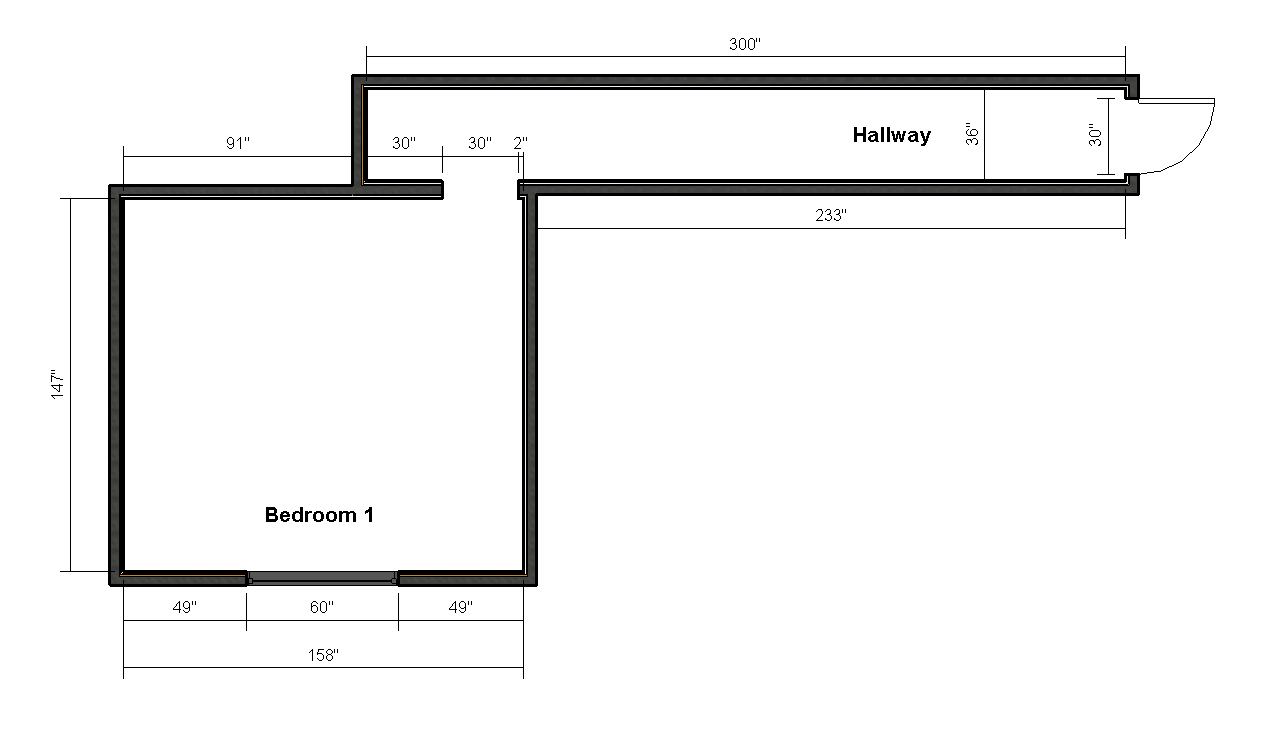
\includegraphics[width=\textwidth]{Figures/Structures/floorplan.png}
\caption{Floor Plan}
\label{fig:floorplan}
\end{figure}

Since these room fire experiments were intended to examine room and contents fires, and not structure fires, the walls of the fire room (Bedroom 1) and hallway were lined with two layers of gypsum board: a surface layer of 1/2~in. board and a base layer, also of 1/2~in. board. The exterior wall outside of the bedroom 1 window was covered with cement board to limit exterior fire spread. The exterior of bedroom 1 can be seen in Figure~\ref{fig:bedroomext}, and the interior hallway with finished drywall can be seen in Figure~\ref{fig:inthallway}.

\begin{figure}[H]
\centering
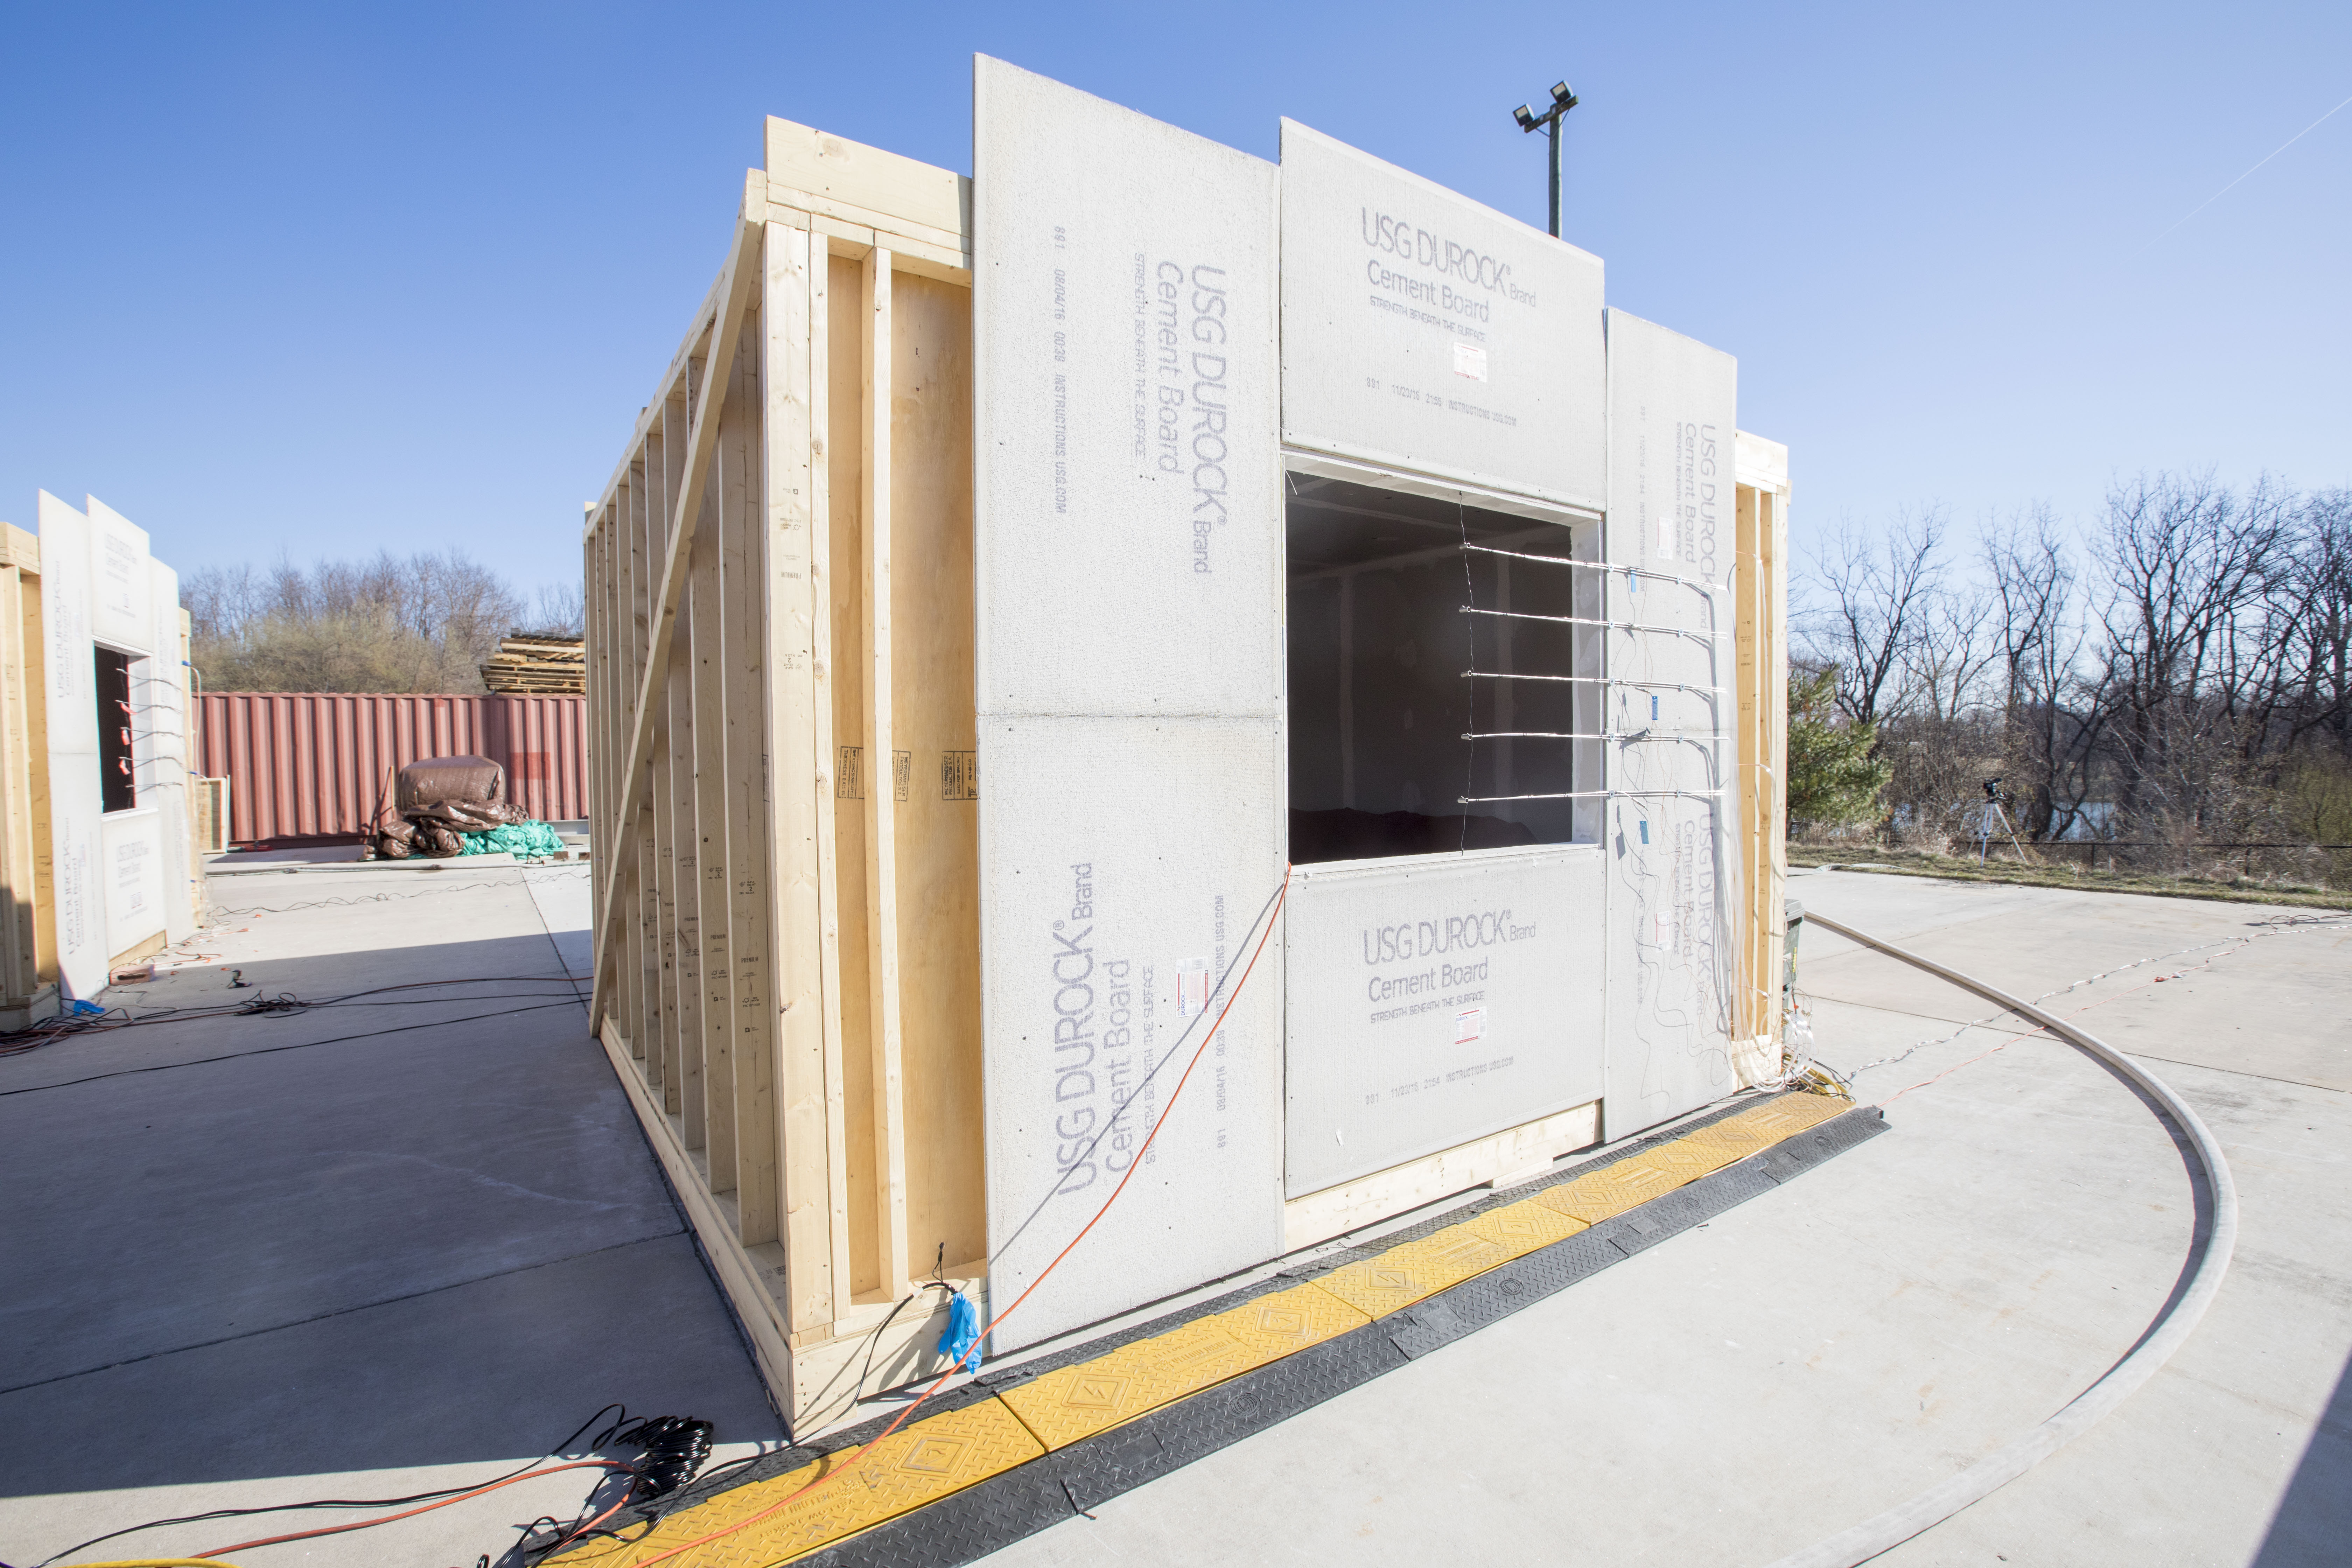
\includegraphics[width=\textwidth]{Figures/Structures/bedroomext.png}
\caption{Exterior of Bedroom 1}
\label{fig:bedroomext}
\end{figure}

\begin{figure}[H]
\centering
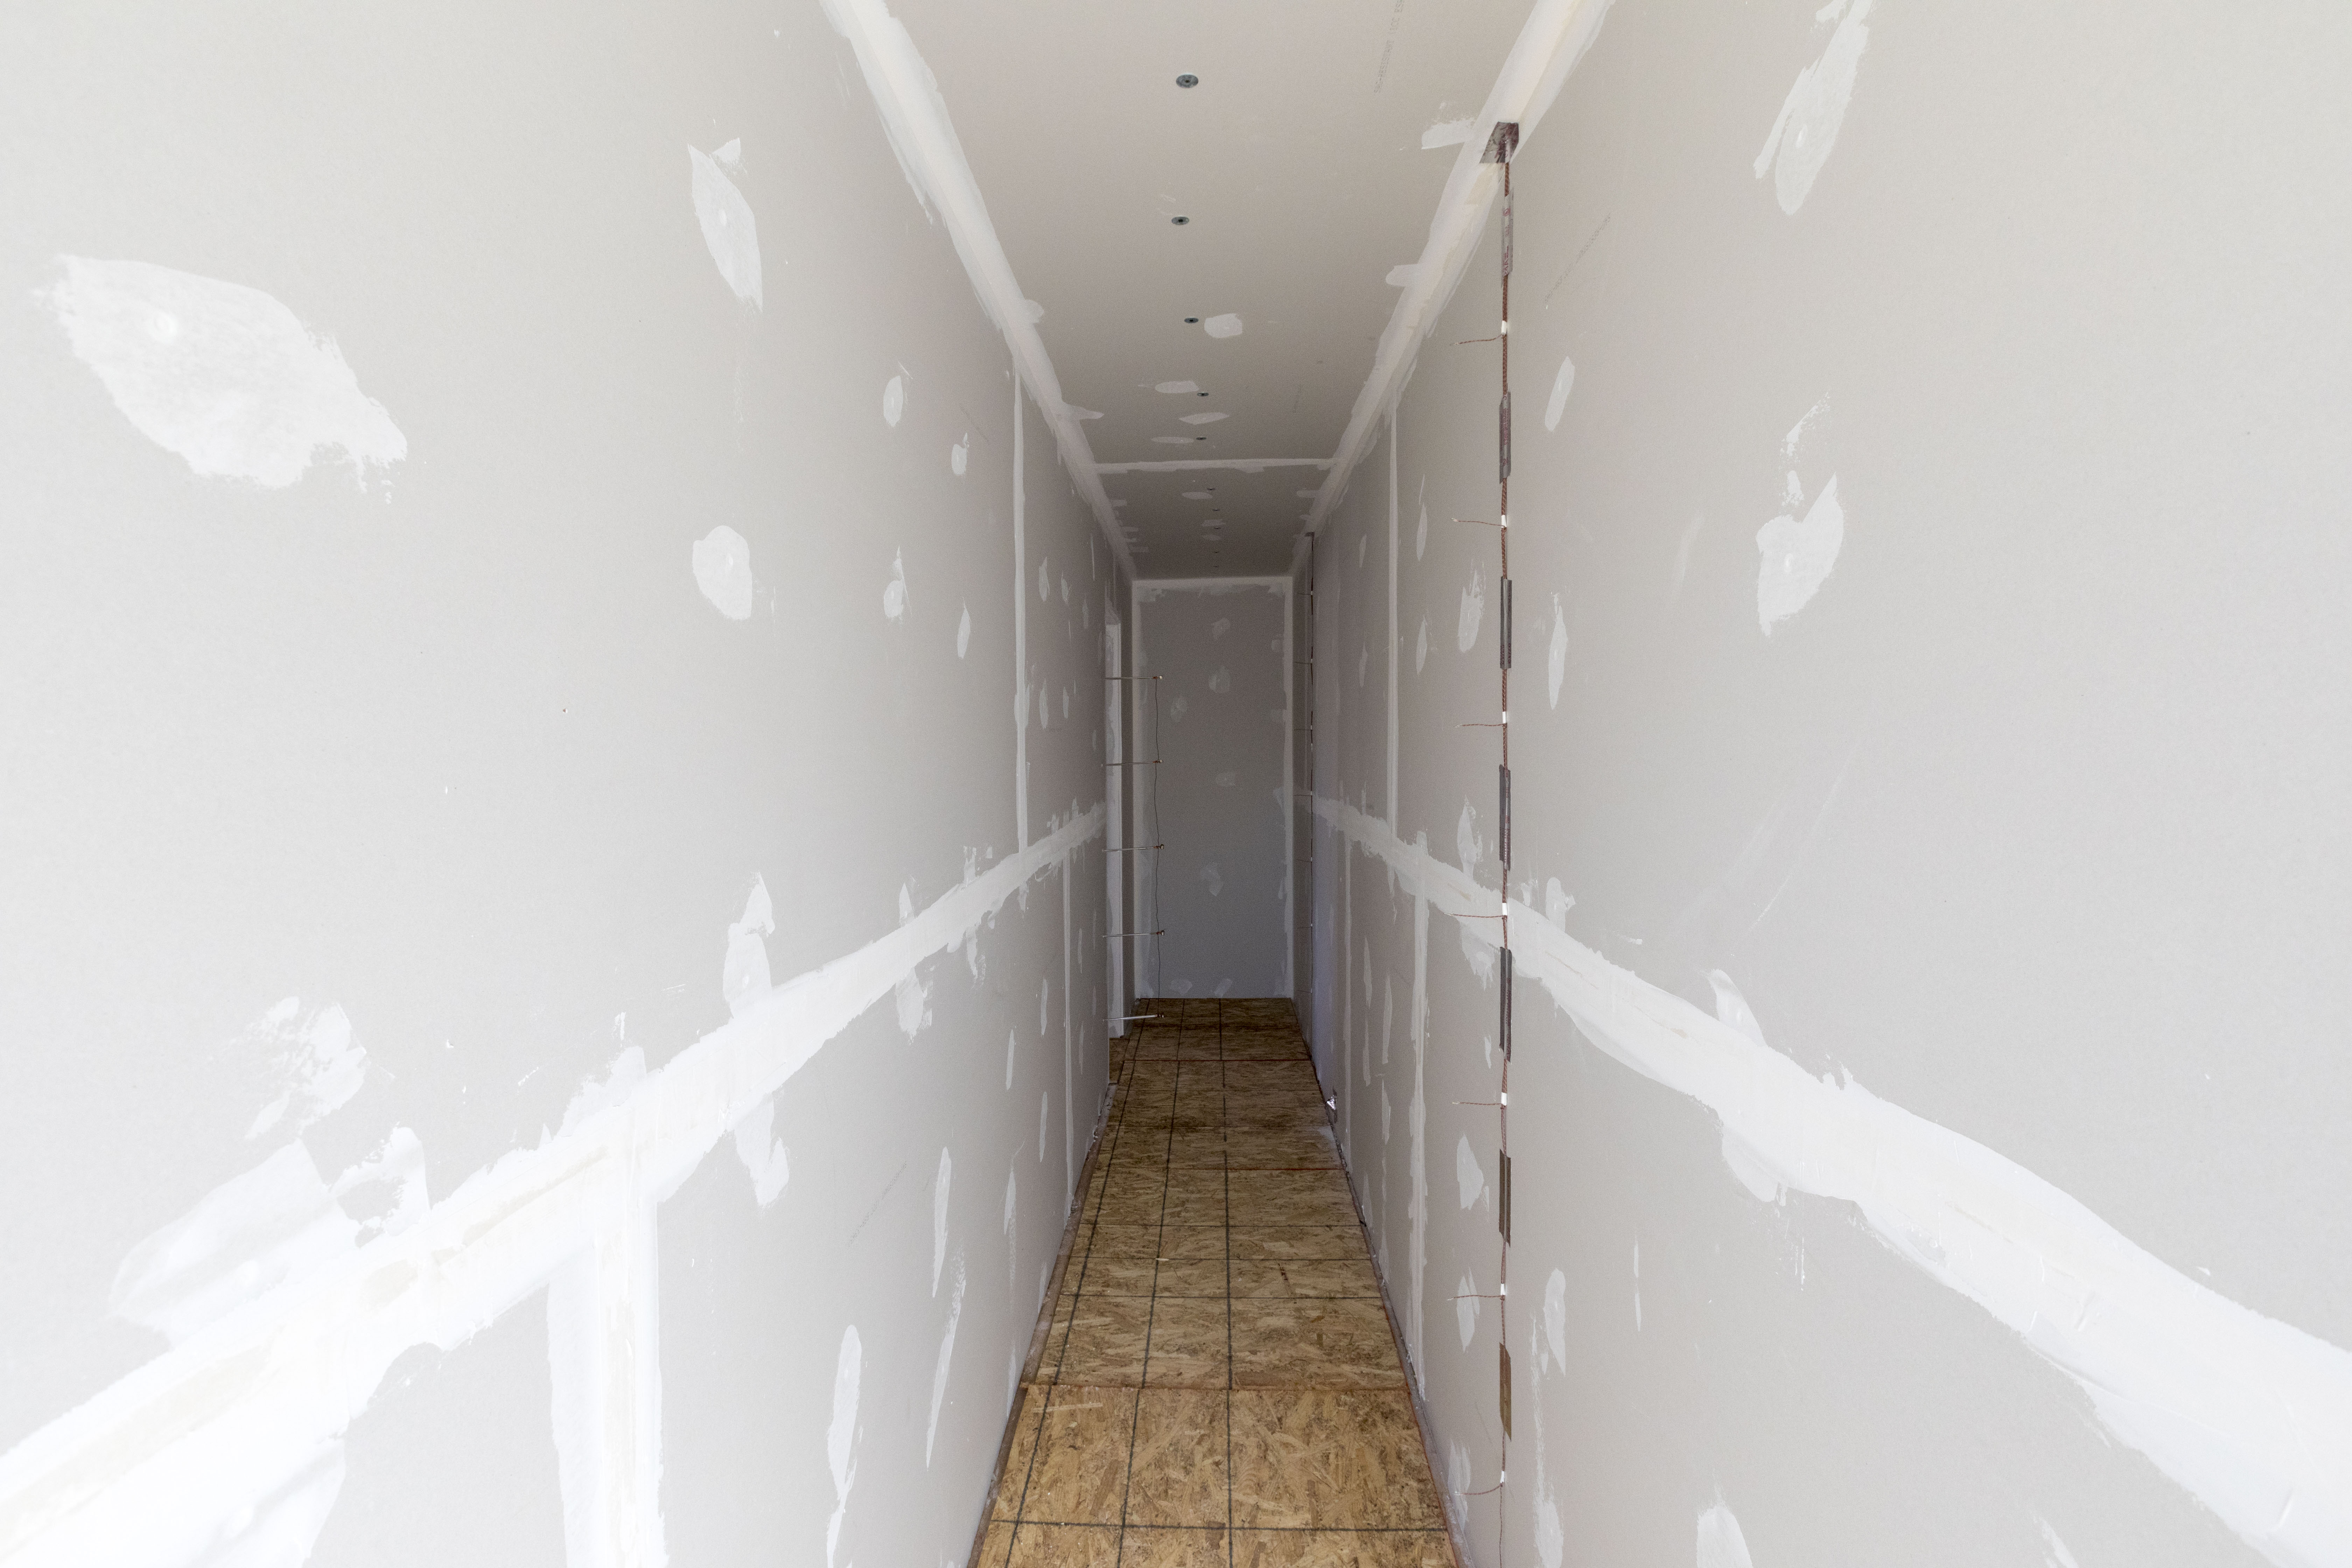
\includegraphics[width=\textwidth]{Figures/Structures/inthallway.png}
\caption{Interior Hallway}
\label{fig:inthallway}
\end{figure}

\paragraph{Air Leakage in the Structure}

The leakage of the structure was determined through the use of a blower door test in accordance with ANSI E1872. A retotec model 5101 blower door was used in accordance with the user manual~\cite{RetroTecManual}.

The standard for leakage of a structure is determined by the IECC. In 2009 the leakage for all climate zones could not exceed 7 air changes per hour. In the 2012 version of the standard the requirement was increased to less than or equal 5 air changes per hour for climate zones 1 and 2 and less than 3 air changes per hour for climate zones 3 $-$ 8.  The structure had a leakage rate of \hl{25 air changes per hour} making it more consistent with leakage found in homes constructed prior to the 2009 IECC. 

Another measure of the leakage, Equivalent Leakage Area (ELA) was also calculated through the use of the blower door. This measurement takes into account all the leakage in a structure, as a flow, and calculates an opening size required to permit that flow. The structures used had an equivalent leakage area of \hl{1.2 $ft^2$}. This is equivalent to having a \hl{15"} diameter hole in the structure. In reality this area is distributed throughout all the smaller openings like those found around windows; however, this calculation allows for the visualization of the size of opening required to provide the leakage rate found in the test fixture utilized. 

\section*{Furnishings}

Furniture was acquired for the experiments such that each room of furniture was the same from experiment to experiment. Descriptions and dimensions for all of the furniture used are in Table~\ref{FurnitureTable}. Images of each piece of furniture can be seen in Figure~\ref{fig:FurnitureImages}.

\renewcommand{\arraystretch}{1.5}
\begin{table}[H]
	\centering
	\caption{Furniture Dimensions and Weight}
		\begin{tabular}[c]{|c|c|c|c|}
			\hline
			\textbf{Item} & \textbf{Length (in.)} & \textbf{Width (in.)} & \textbf{Height (in.)} \\ \hline \hline
			Sofa & 89 & 39 & 40 \\ \hline
			Mattress & 75 & 54 & 7.5 \\ \hline
			Box Spring & 75 & 54 & 12 \\ \hline
		\end{tabular}
	\label{FurnitureTable}
\end{table}

% \begin{figure}
% 	\centering
% 	\begin{tabular}[c]{c c}
% 		\subfloat[Sofa]{\includegraphics[width=6cm]{Figures/Furniture/sofa.jpg}} &
% 		\subfloat[Mattress \& Boxspring]{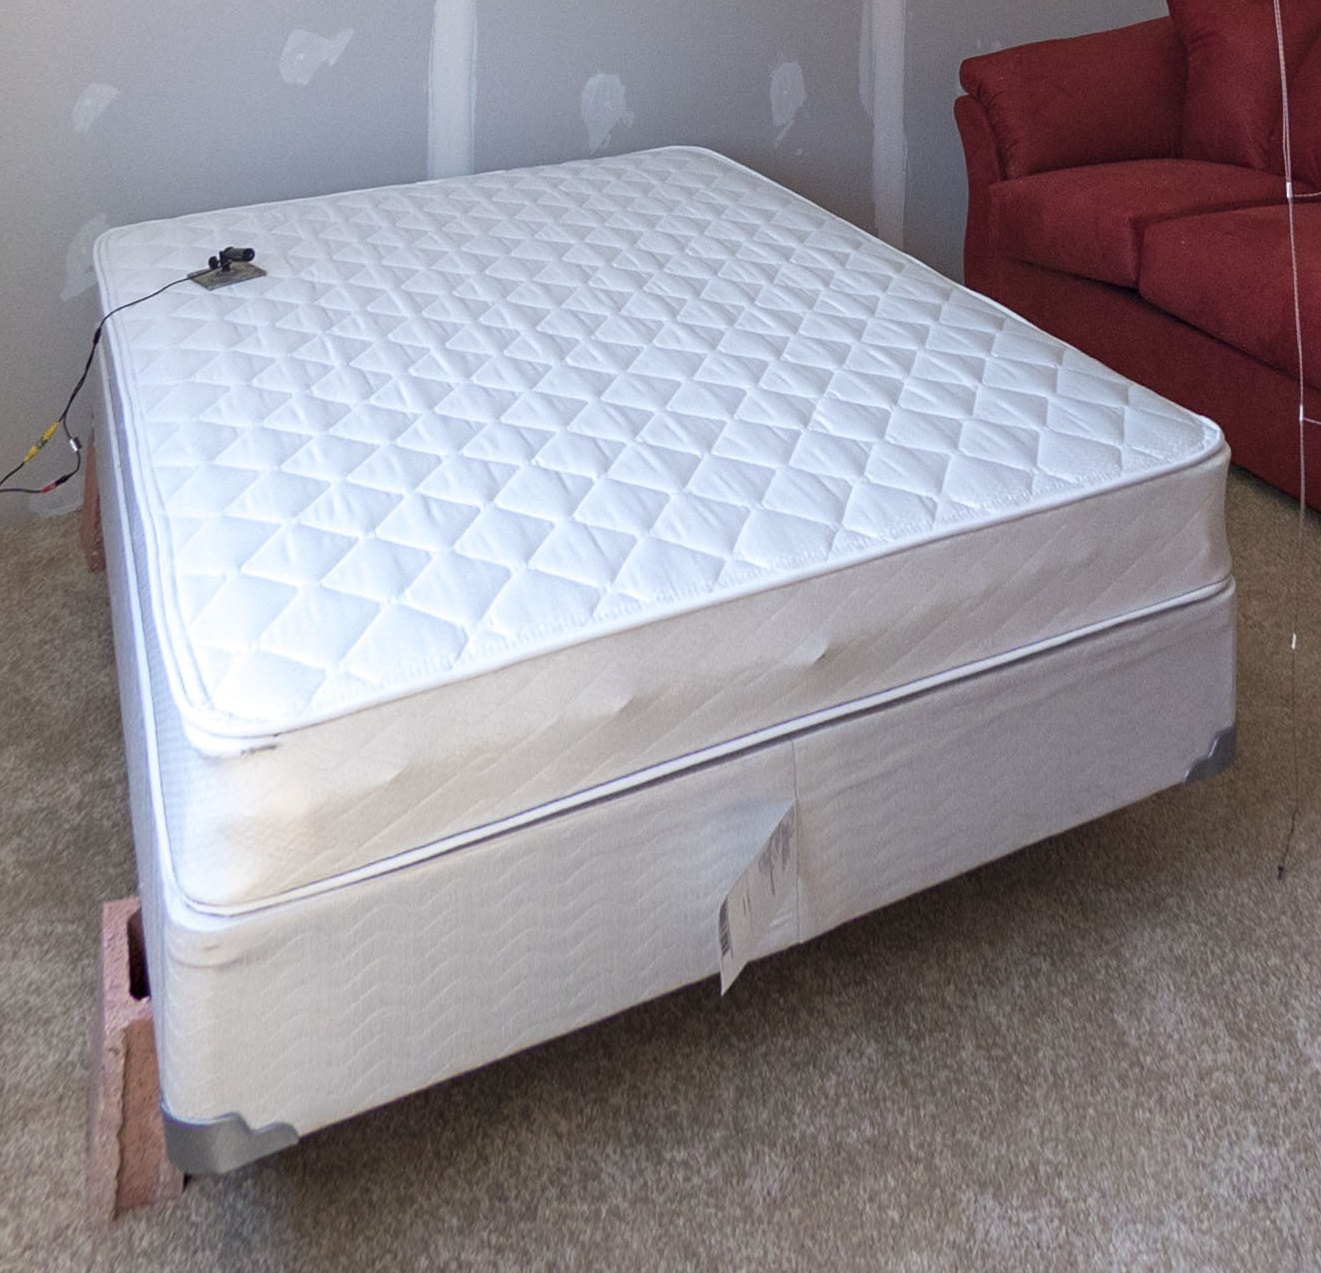
\includegraphics[width=6cm]{Figures/Furniture/bed.jpg}} \\
% 	\end{tabular}
% 	\caption{Furniture Images}
% 	\label{fig:FurnitureImages}
% \end{figure}

\begin{figure}[ht]
  \centering
  \begin{subfigure}[Sofa]{0.5\linewidth}
    \centering\includegraphics[width=6cm]{Figures/Furniture/sofa.jpg}
    \caption{\label{fig:Sofa}}
  \end{subfigure}
  \begin{subfigure}[Bed]{0.5\linewidth}
    \centering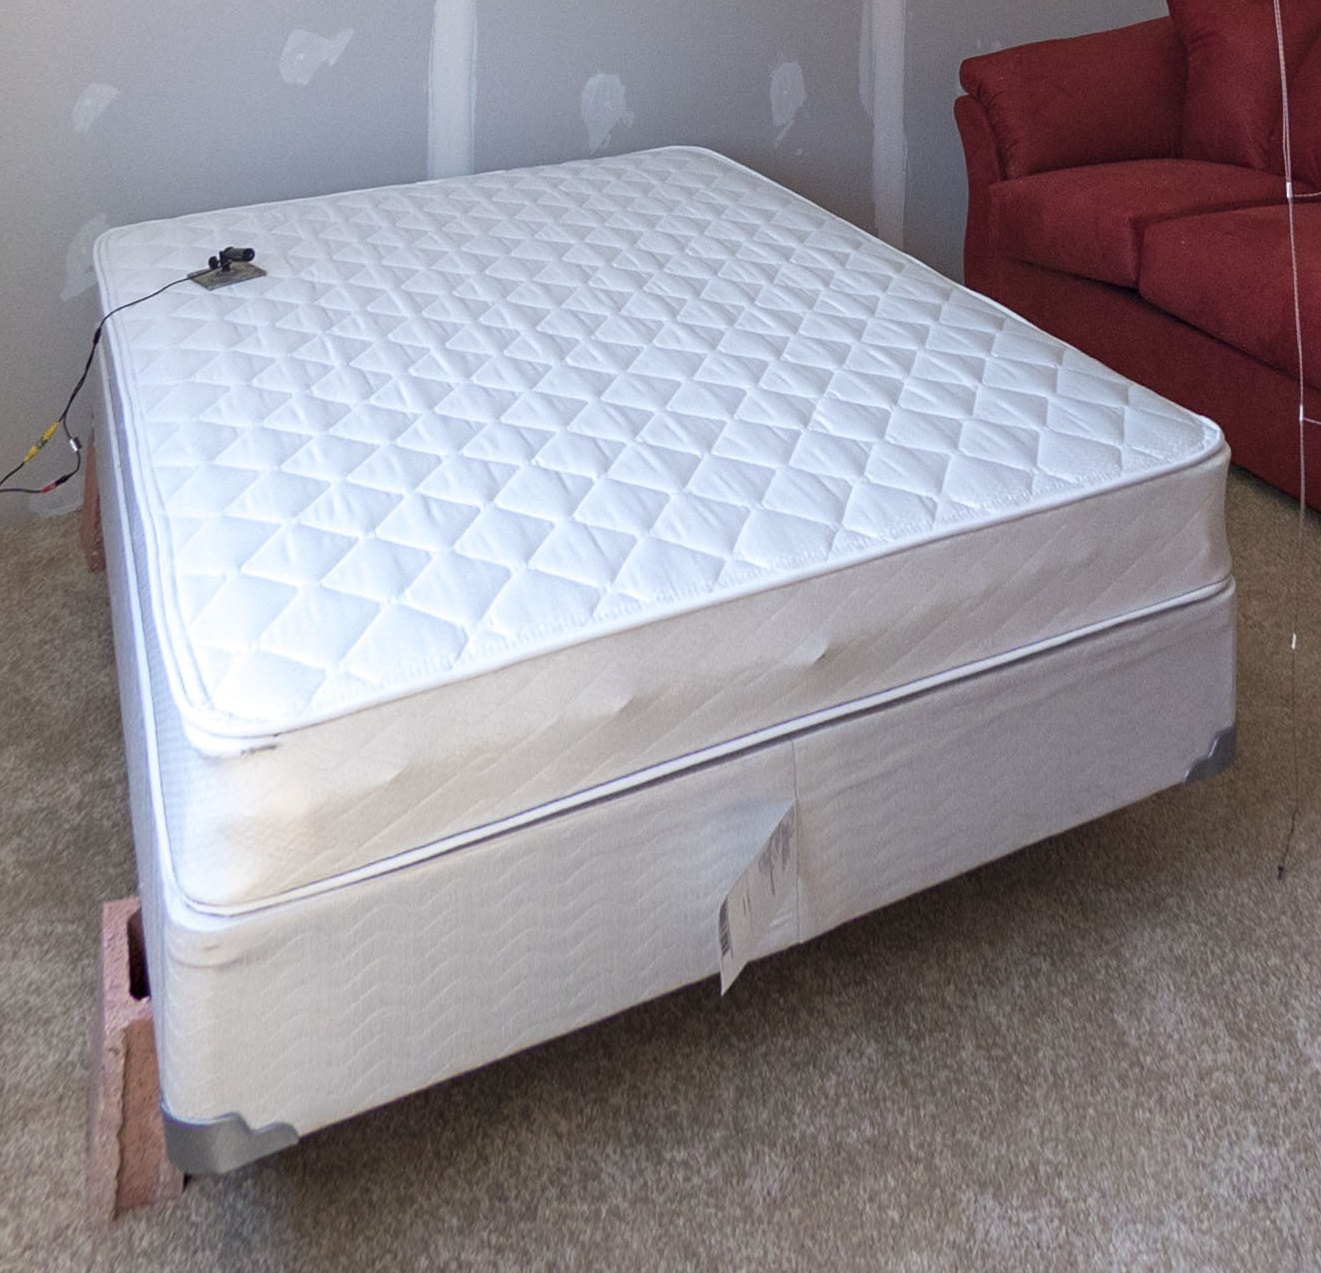
\includegraphics[width=6cm]{Figures/Furniture/bed.jpg}
    \caption{\label{fig:Bed}}
  \end{subfigure}
  \caption{Picture~\subref{fig:Sofa} shows the sofa and Picture~\subref{fig:Bed} shows the mattress and boxspring used as furnishings for these experiments.}
  \label{fig:FurnitureImages}
\end{figure}

For Experiment 1, the bedroom in the structure was furnished with two full-size sofas. The floor was covered with 7/16~in. oriented strand board (OSB). For Experiments 2 through 6, the bedroom in the structure was furnished with a mattress \& boxspring (full size) and two full-size sofas. The floor was covered with 7/16~in. OSB, polyurethane foam padding, and polyester carpet. Figures~\ref{fig:Exp1Furniture} and~\ref{fig:Exp2to6Furniture} show the bedroom furniture setup for all of the experiments conducted.

\begin{figure}[H]
	\centering
	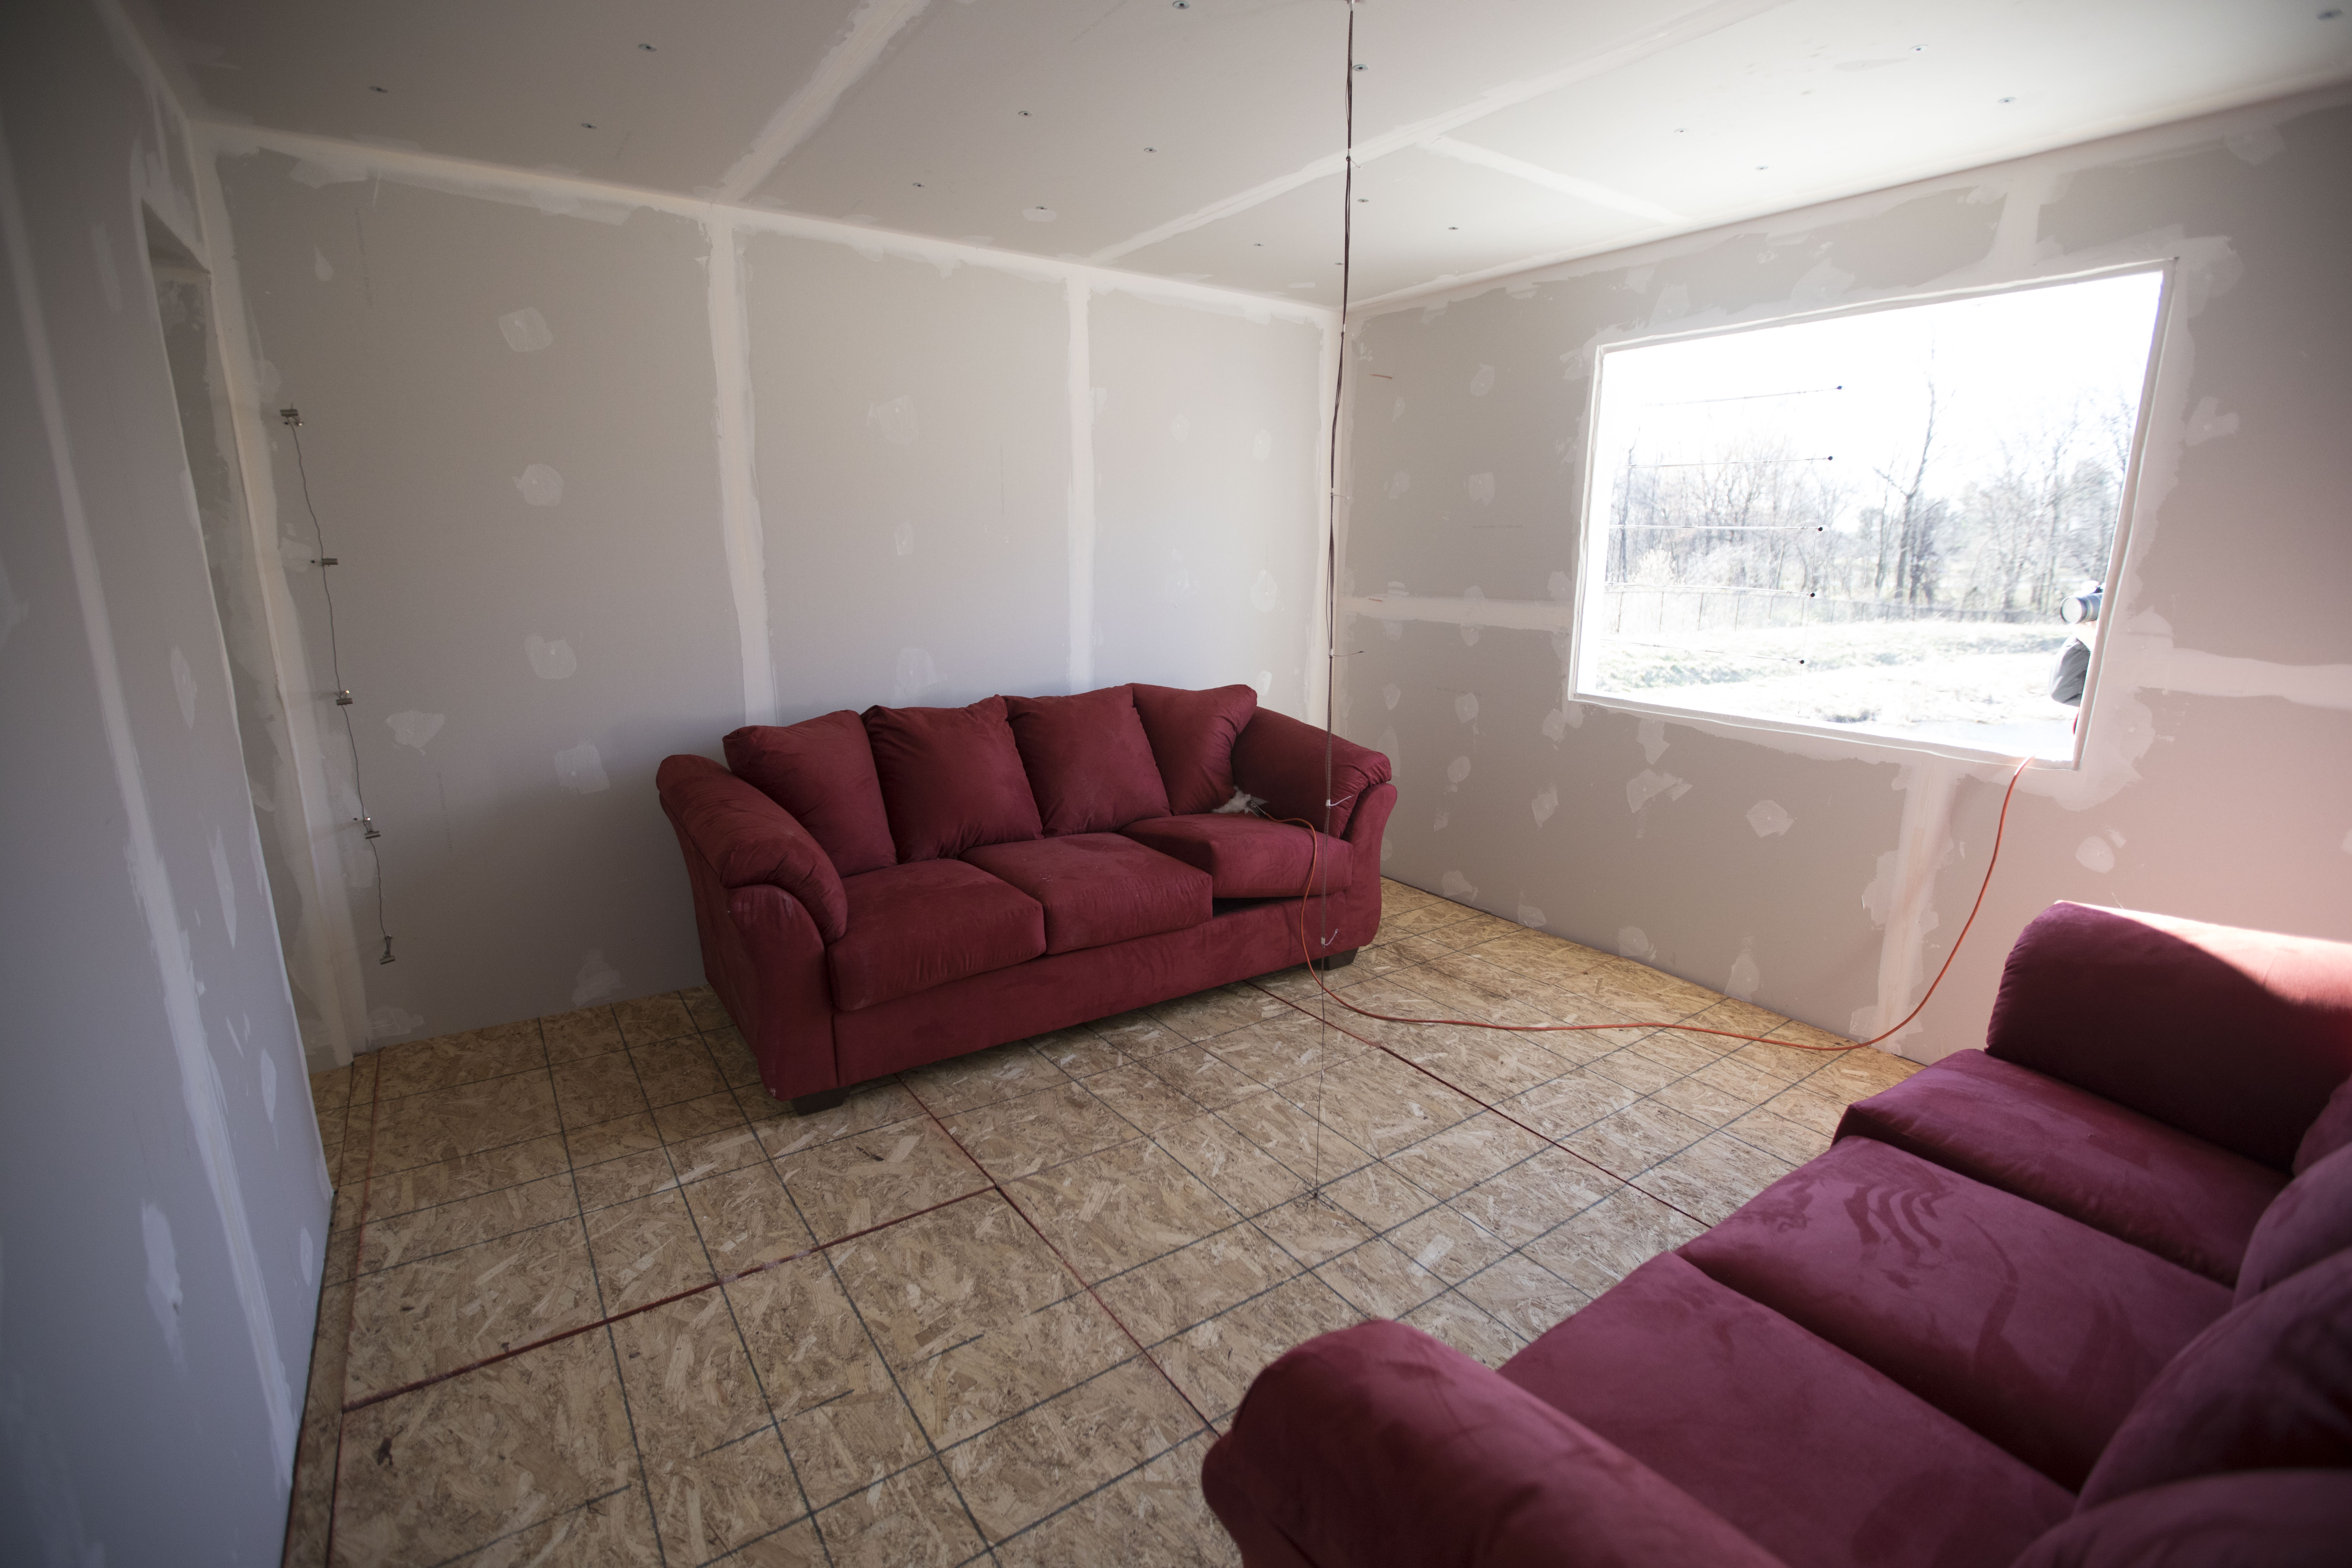
\includegraphics[width=\textwidth]{Figures/Furniture/Exp1Furniture.jpg}
	\caption{Experiment 1 Furniture Layout}
	\label{fig:Exp1Furniture}
\end{figure}

\begin{figure}[H]
	\centering
	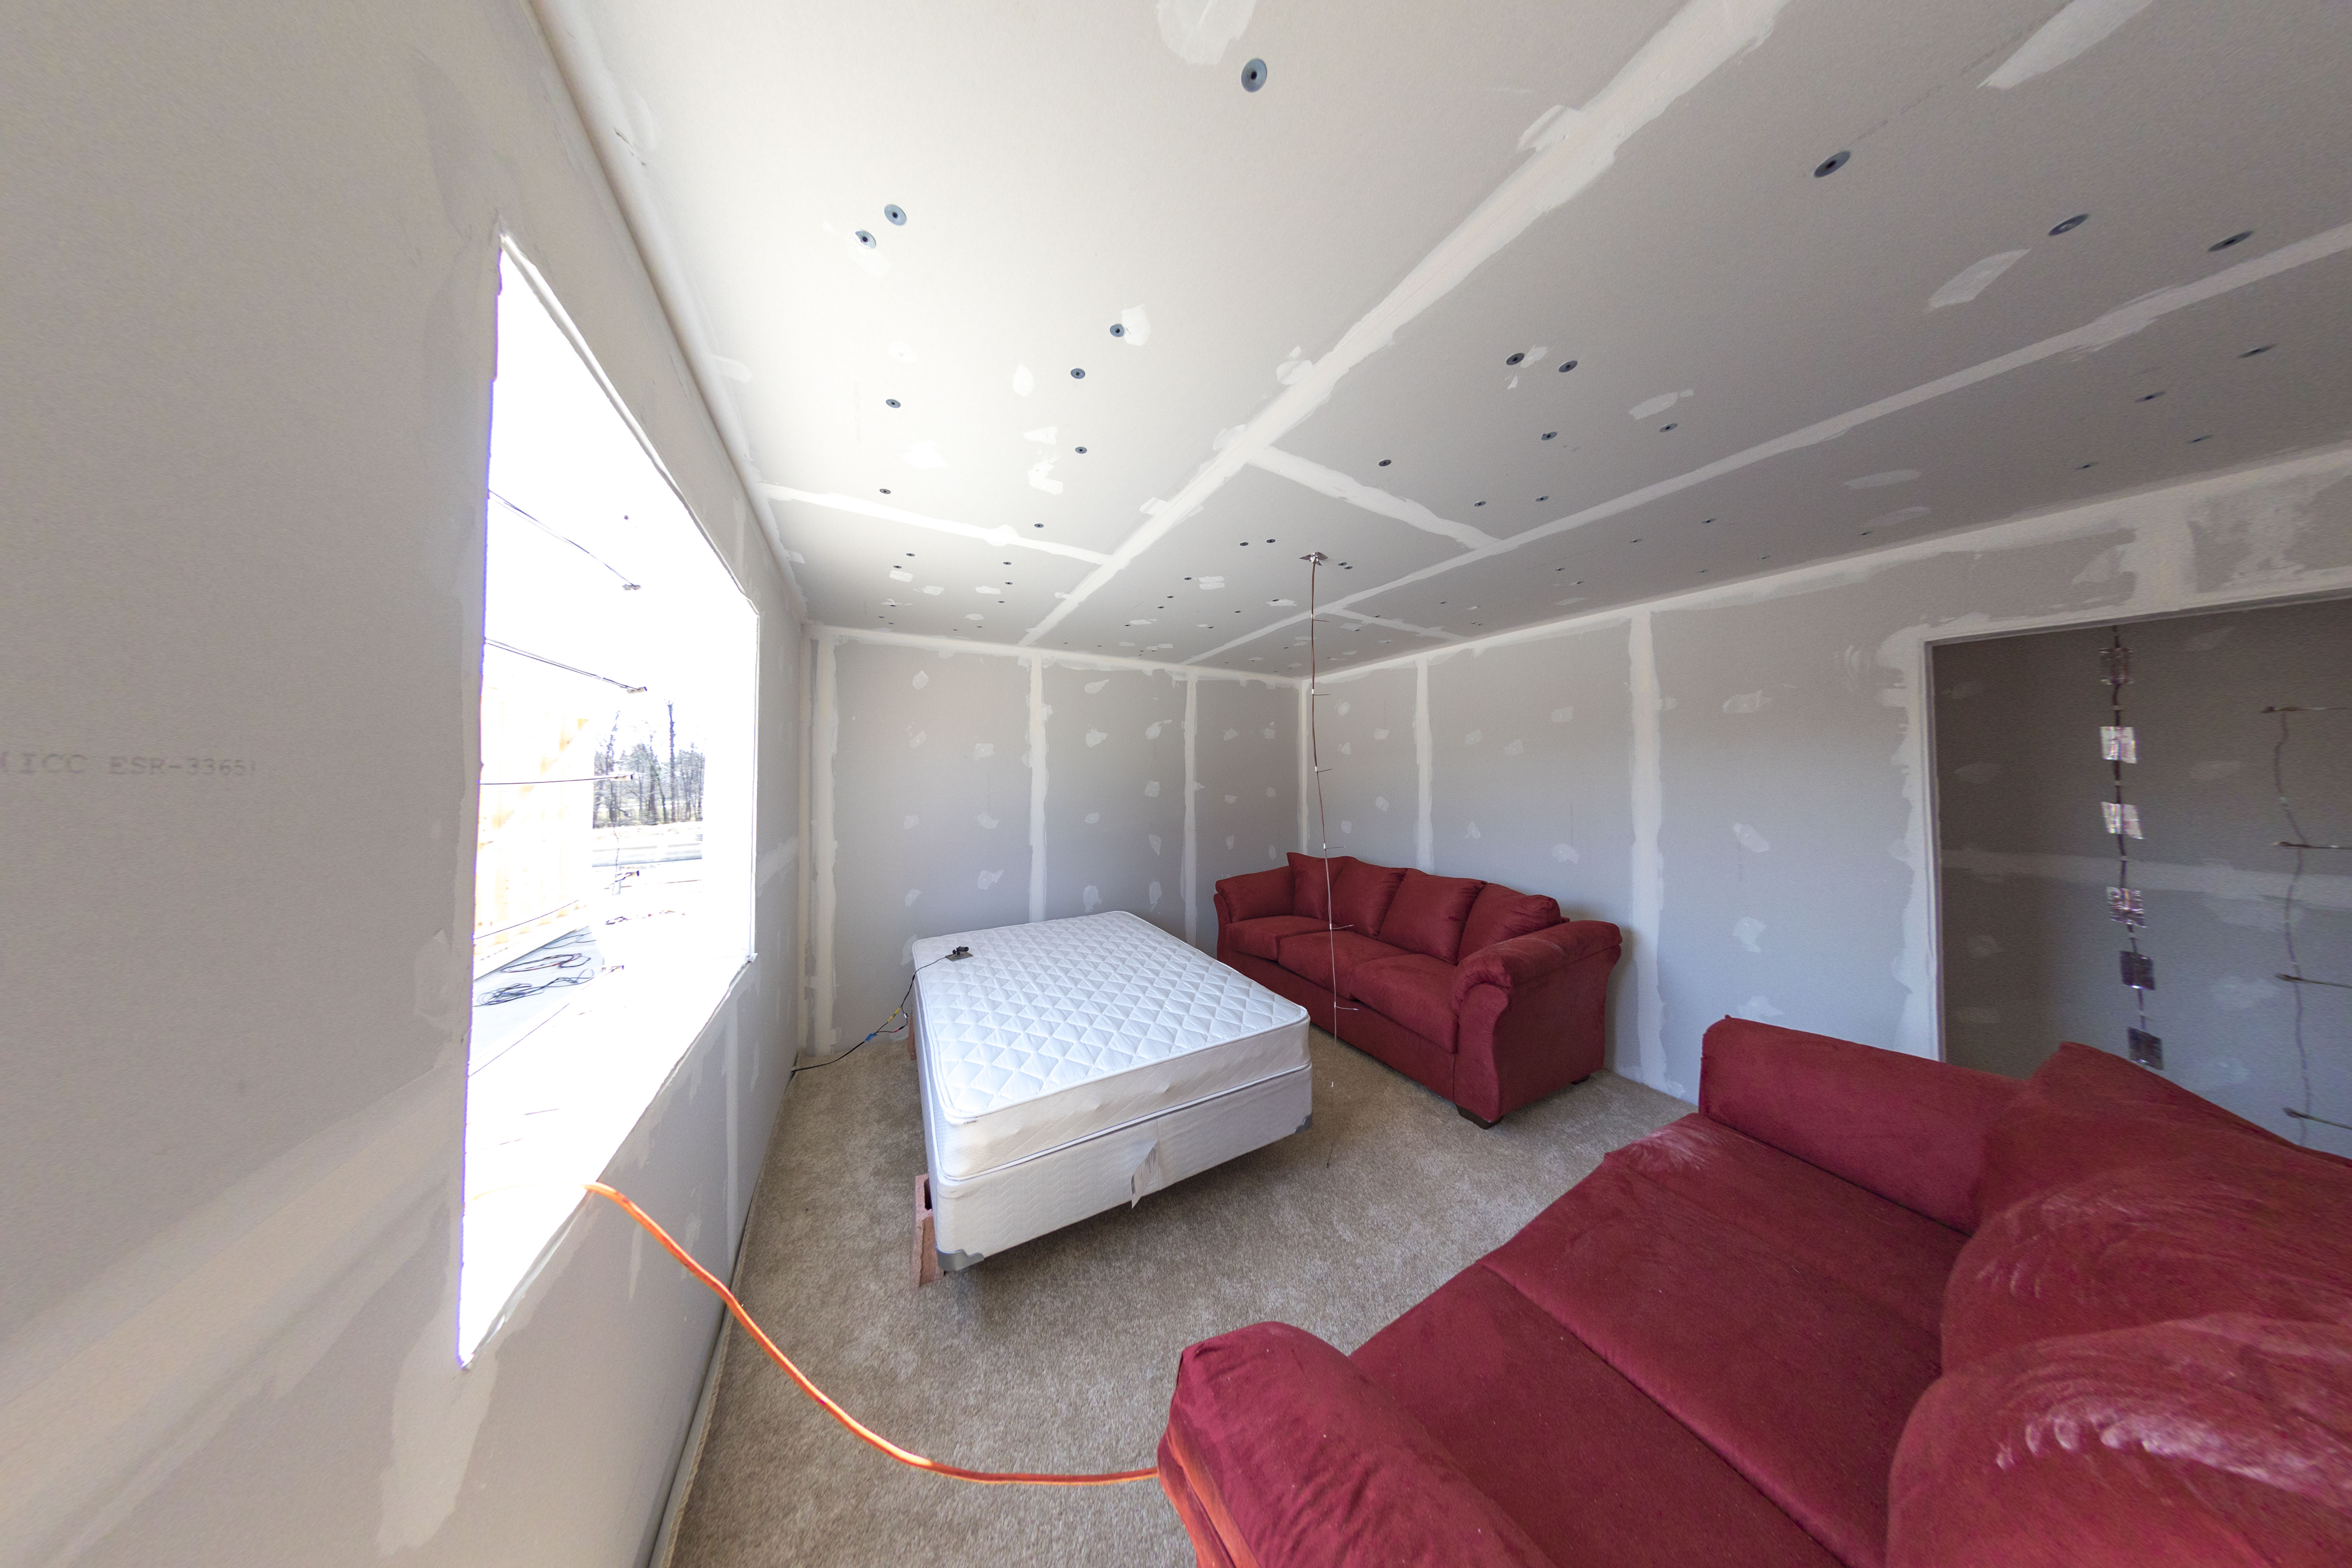
\includegraphics[width=\textwidth]{Figures/Furniture/Exp2to6Furniture.jpg}
	\caption{Experiments 2-6 Furniture Layout}
	\label{fig:Exp2to6Furniture}
\end{figure}

For exact locations of furniture within the structure, see Figure~\ref{fig:Exp1FurnitureDim} and Figure~\ref{fig:Exp2to6FurnitureDim}. 

\begin{figure}[H]
	\centering
	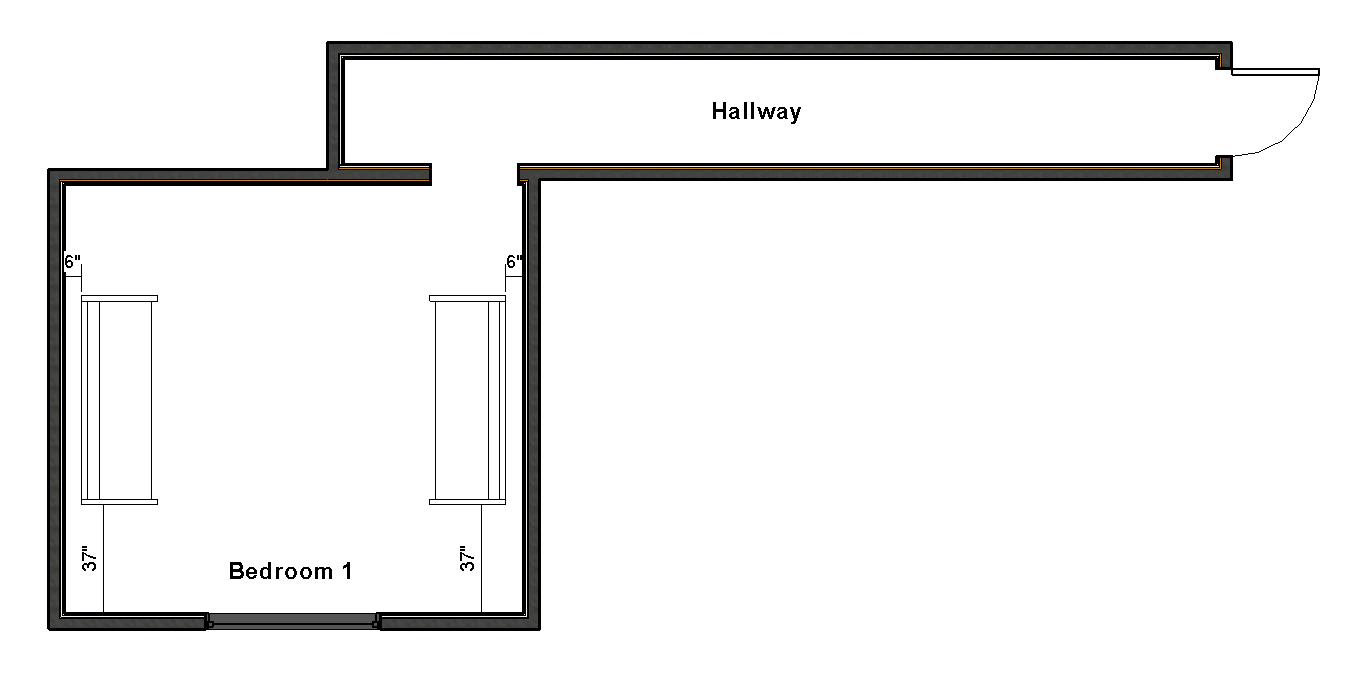
\includegraphics[width=\textwidth]{Figures/Furniture/Exp1FurnitureDimensions.png}
	\caption{Experiment 1 Furniture Layout}
	\label{fig:Exp1FurnitureDim}
\end{figure}

\begin{figure}[H]
	\centering
	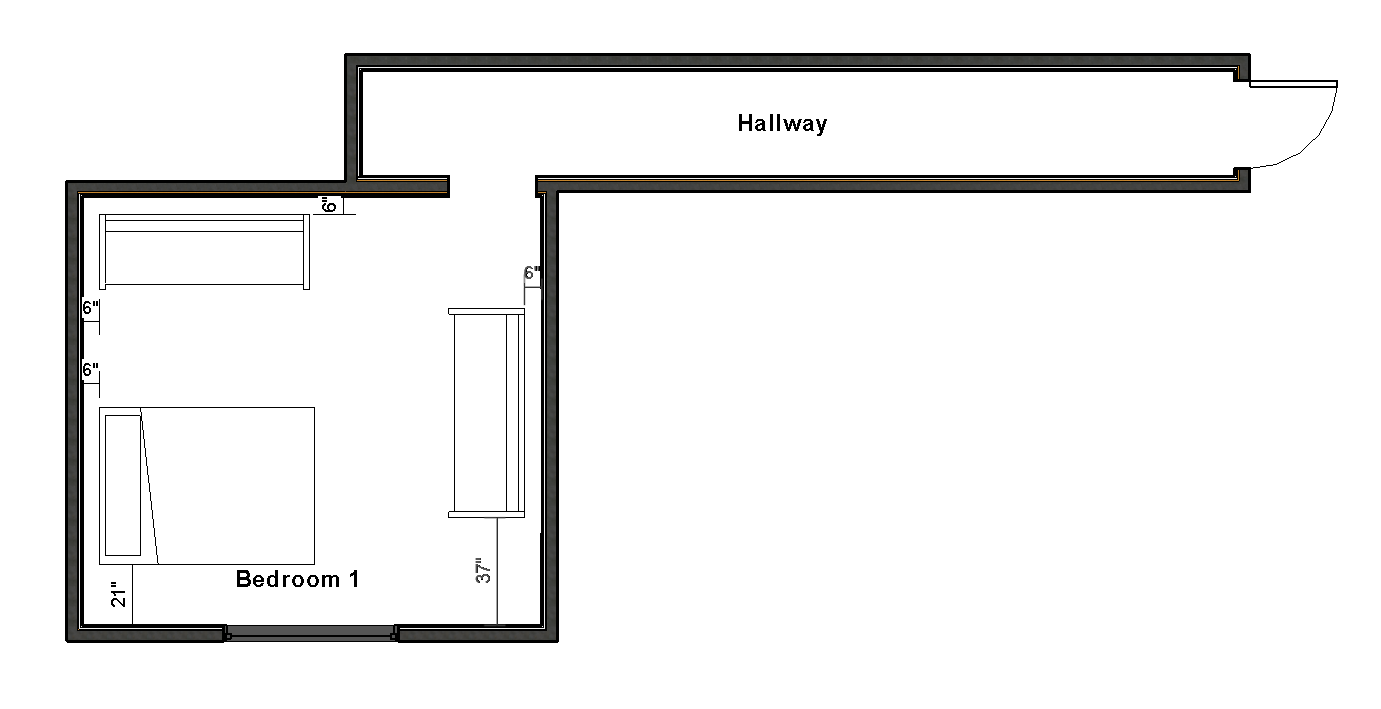
\includegraphics[width=\textwidth]{Figures/Furniture/Exp2to6FurnitureDimensions.png}
	\caption{Experiment 2-6 Furniture Layout}
	\label{fig:Exp2to6FurnitureDim}
\end{figure}

\section*{Measurement Locations}

The test fixture was instrumented with temperature, air flow, and pressure sensors. Temperature was measured via Type K thermocouples built into an array. Each array contained 7 measurement locations at 1~ft., 2~ft., 3~ft., 4~ft., 5~ft., 6~ft., and 7~ft. above the floor level. An array was located in the center of the bedroom and in three locations spaced equally along the length of the hallway. Air flow was measured via bi-directional probes. The bedroom 1 doorway (just inside the bedroom and just outside the bedroom) and the entrance of the hallway were instrumented with five bi-directional probes arrayed vertically along the center line at 13.75~in., 27.5~in., 41.25~in., 55~in., and 68.75~in. above the floor. In addition, the bedroom 1 window was instrumented with five bi-directional probes arrayed vertically along the center line at 7~in., 15~in., 23~in., 31~in., and 39~in. above the window sill. Pressure was recorded through a differential pressure transducer in the bedroom as well as the entrance to the hallway at 1~ft., 4~ft., and 7~ft. above the floor. 

The location of each sensor within the structure is shown in Figure~\ref{fig:InstrumentDim}.

\begin{figure}[H]
	\centering
	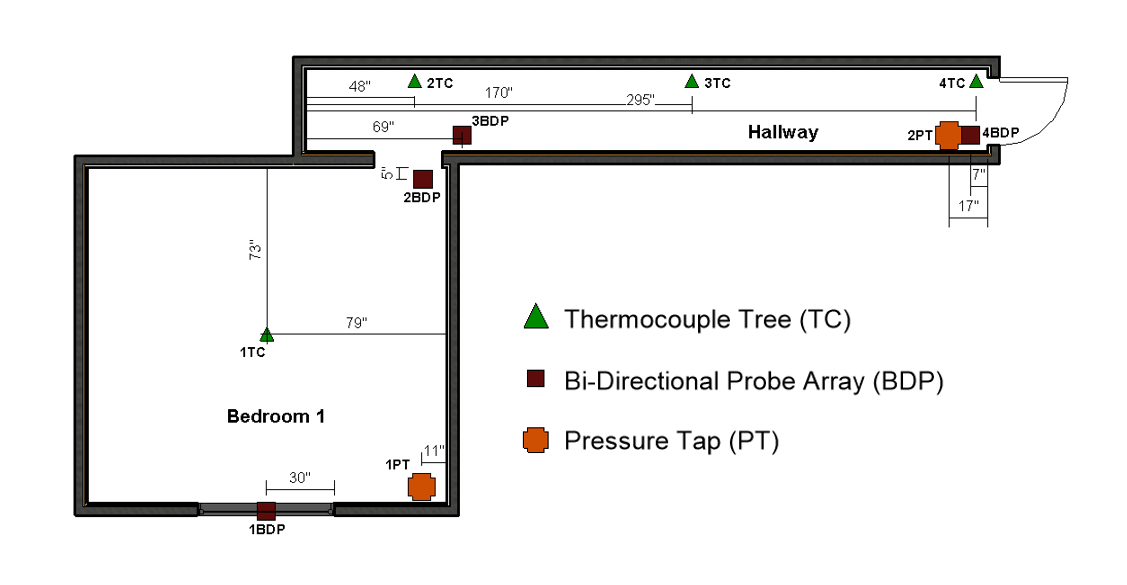
\includegraphics[width=\textwidth]{Figures/Instrumentation/Instrument_Dimensions.png}
	\caption{Instrumentation Layout}
	\label{fig:InstrumentDim}
\end{figure}

\clearpage

\chapter{Test Descriptions}

\section*{Entrainment Experiments}

\paragraph{Entrainment Experiments~1 and~2} \mbox{}

Entrainment Experiments~1 and 2 followed the same sequence of interventions listed in Table~\ref{Table:EntExp1_and_2_Interventions}. The experiments involved flowing a straight stream in the fixed position, then a straight stream in the WCW pattern [BE SURE TO EXPLAIN IN EARLIER SECTION], followed by a narrow fog stream in the fixed position and a narrow fog in the `O' pattern. These four different configurations were used at three different locations, referred to as `start hall', `mid hall', and `end hall', which corresponded to distances of 4~ft, 12~ft, and 20~ft from the interior side of the entrance doorway of the hall. The bedroom window was opened for the entire duration of the experiments.

% \begin{figure}[H]
% 	\centering
% 	\includegraphics[width=5in]{Howard_EntExp_1}
% 	\caption{Entrainment Experiments~1 and~2 Configuration}
% 	\label{fig:EntExp1_and_2_Config}
% \end{figure}

\begin{table}[H]
	\centering
	\caption{Entrainment Experiments~1 and~2 Interventions}
	\begin{tabular}{|c|c|c|} 
		\hline
		Exp.~1 Time 	& 	Exp.~2 Time 	& 	Intervention 	\\ \hline \hline
			00:00 		& 	00:00  			& 	Background	\\ \hline
			01:00	 	& 	01:00  			& 	Straight Stream Fixed Start Hall 	\\ \hline
			02:00		& 	02:00  			& 	Straight Stream WCW Start Hall 	\\ \hline
			03:00	 	& 	03:00  			& 	Narrow Fog Fixed Start Hall 	\\ \hline
			04:00		& 	04:00  			& 	Narrow Fog `O' Start Hall 	\\ \hline
			05:00		& 	05:00  			&	No Action 	\\ \hline
			06:00		& 	06:00  			& 	Straight Stream Fixed Mid Hall 	\\ \hline
			07:00		& 	07:00  			& 	Straight Stream WCW Mid Hall 	\\ \hline
			08:00		& 	08:00  			& 	Narrow Fog Fixed Mid Hall 	\\ \hline
			09:00		& 	09:00  			& 	Narrow Fog `O' Mid Hall 	\\ \hline
			10:00		& 	10:00  			& 	No Action 	\\ \hline
			13:00		& 	16:00  			& 	Straight Stream Fixed End Hall 	\\ \hline
			14:00		& 	17:00  			& 	Straight Stream WCW End Hall 	\\ \hline
			15:00		& 	18:00  			& 	Narrow Fog Fixed End Hall 	\\ \hline
			16:00		& 	19:00  			& 	Narrow Fog `O' End Hall 	\\ \hline
			17:00		& 	20:00  			& 	No Action 	\\ \hline
			18:00		& 	21:00  			& 	End Experiment 	\\ \hline
	\end{tabular}
	\label{Table:EntExp1_and_2_Interventions}
\end{table}

\FloatBarrier

\paragraph{Entrainment Experiment~3} \mbox{}
Entrainment Experiment~3 followed the same order of events as Entrainment Experiments~1 and~2. The only difference for Entrainment Experiment~3 was that the bedroom window was closed for the entire duration of the experiment. Entrainment Experiment~3 was conducted to determine the effect of venting ahead of the hose stream on air entrainment within a structure. 

% \begin{figure}[H]
% 	\centering
% 	\includegraphics[width=5in]{Howard_EntExp_3}
% 	\caption{Entrainment Experiment~3 Configuration}
% 	\label{fig:EntExp3_Config}
% \end{figure}

\begin{table}[H]
	\centering
	\caption{Entrainment Experiment~3 Interventions}
	\begin{tabular}{|c|c|} 
		\hline
		Time 	& 	Intervention 	\\ \hline \hline
		00:00 	&	Background 	\\ \hline
		02:00 	&	Straight Stream Fixed Start Hall 	\\ \hline
		04:00 	&	Straight Stream WCW Start Hall 	\\ \hline
		05:00 	&	Narrow Fog Fixed Start Hall 	\\ \hline
		06:00 	&	Narrow Fog `O' Start Hall 	\\ \hline
		07:00 	&	No Action 	\\ \hline
		08:00 	&	Straight Stream Fixed Mid Hall 	\\ \hline
		09:00 	&	Straight Stream WCW Mid Hall 	\\ \hline
		10:00 	&	Narrow Fog Fixed Mid Hall 	\\ \hline
		11:00 	&	Narrow Fog `O' Mid Hall 	\\ \hline
		12:00 	&	No Action 	\\ \hline
		14:00 	&	Straight Stream Fixed End Hall 	\\ \hline
		15:00 	&	Straight Stream WCW End Hall 	\\ \hline
		16:00 	&	Narrow Fog Fixed End Hall 	\\ \hline
		17:00 	&	Narrow Fog Fixed End Hall 	\\ \hline
		18:22 	&	Narrow Fog `O' End Hall 	\\ \hline
		19:22 	&	No Action 	\\ \hline
		20:22 	&	End Experiment 	\\ \hline
	\end{tabular}
	\label{Table:EntExp3_Interventions}
\end{table}

\FloatBarrier

\paragraph{Entrainment Experiment~4} \mbox{}

% \begin{figure}[H]
% 	\centering
% 	\includegraphics[width=5in]{Howard_EntExp_4}
% 	\caption{Entrainment Experiment~4 Configuration}
% 	\label{fig:EntExp4_Config}
% \end{figure}

\begin{table}[H]
	\centering
	\caption{Entrainment Experiment~4 Interventions}
	\begin{tabular}{|c|c|} 
		\hline
 		Time 	& 	Intervention 	\\ \hline \hline
 		00:00	&	Background 	\\ \hline
		02:00	&	Straight Stream Fixed Max Angle 	\\ \hline
		03:00	&	Straight Stream `O' Max Angle 	\\ \hline
		04:00	&	Straight Stream Fixed Mid Ceiling 	\\ \hline
		05:00	&	Straight Stream `O' Mid Ceiling 	\\ \hline
		06:00	&	Straight Stream Fixed Out Window 	\\ \hline
		07:00	&	Straight Stream `O' Out Window 	\\ \hline
		08:00	&	Straight Stream Room Sweep 	\\ \hline
		09:00	&	No Action 	\\ \hline
		18:00	&	Narrow Fog Fixed Max Angle 	\\ \hline
		19:00	&	Narrow Fog `O' Max Angle 	\\ \hline
		20:02	&	Narrow Fog Fixed Mid Ceiling 	\\ \hline
		21:03	&	Narrow Fog `O' Mid Ceiling 	\\ \hline
		22:03	&	Narrow Fog Fixed Out Window 	\\ \hline
		23:03	&	Narrow Fog `O' Out Window 	\\ \hline
		24:03	&	Narrow Fog Room Sweep 	\\ \hline
		25:04	&	No Action 	\\ \hline
		27:03	&	End Experiment 	\\ \hline
	\end{tabular}
	\label{Table:EntExp4_Interventions}
\end{table}

\FloatBarrier

\paragraph{Entrainment Experiments~5 and~6} \mbox{}

% \begin{figure}[H]
% 	\centering
% 	\includegraphics[width=5in]{Howard_EntExp_5}
% 	\caption{Entrainment Experiments~5 and~6 Configuration}
% 	\label{fig:EntExp5_and_6_Config}
% \end{figure}

\begin{table}[H]
	\centering
	\caption{Entrainment Experiments~5 and~6 Interventions}
	\begin{tabular}{|c|c|} 
		\hline
		Exp.~5 \&~6 Time 	& 	Intervention 	\\ \hline \hline
			00:00			& 	Background 	\\ \hline
			02:00			&	At Window Straight Stream Fixed 	\\ \hline
			03:00			&	At Window Straight Stream `O' 	\\ \hline
			04:00			&	At Window Narrow Fog Fixed 	\\ \hline
			05:00			&	At Window Narrow Fog `O' 	\\ \hline
			06:00			&	No Action 	\\ \hline
			07:00			&	6' Straight Stream Fixed 	\\ \hline
			08:00			&	6' Straight Stream `O' 	\\ \hline
			09:00			&	6' Narrow Fog Fixed 	\\ \hline
			10:00			&	6' Narrow Fog `O' 	\\ \hline
			11:00			&	No Action 	\\ \hline
			12:00			&	12' Straight Stream Fixed 	\\ \hline
			13:00			&	12' Straight Stream `O' 	\\ \hline
			14:00			&	12' Narrow Fog Fixed 	\\ \hline
			15:00			&	12' Narrow Fog `O' 	\\ \hline
			16:00			&	No Action 	\\ \hline
			18:00			&	End Experiment 	\\ \hline
	\end{tabular}
	\label{Table:EntExp5_and_6_Interventions}
\end{table}

\FloatBarrier

\paragraph{Entrainment Experiments~8 and~9} \mbox{}

% \begin{figure}[H]
% 	\centering
% 	\includegraphics[width=5in]{Howard_EntExp_8}
% 	\caption{Entrainment Experiments~8 and~9 Configuration}
% 	\label{fig:EntExp8_and_9_Config}
% \end{figure}

\begin{table}[H]
	\centering
	\caption{Entrainment Experiments~8 and~9 Interventions}
	\begin{tabular}{|c|c|} 
		\hline
		Exp.~8 \&~9 Time 	& 	Intervention 	\\ \hline \hline
			00:00 	 		&	Background 	\\ \hline
			02:00 			&	Straight Stream Max Angle Fixed 	\\ \hline
			03:00 			&	Straight Stream Max Angle Sweeping 	\\ \hline
			04:00 			&	No Action 	\\ \hline
			05:00 			&	Narrow Fog Whip 	\\ \hline
			06:00 			&	No Action 	\\ \hline
			08:00 			&	End Experiment 	\\ \hline
	\end{tabular}
	\label{Table:EntExp8_and_9_Interventions}
\end{table}

\FloatBarrier

\paragraph{Entrainment Experiments~10 and~11} \mbox{}

% \begin{figure}[H]
% 	\centering
% 	\includegraphics[width=5in]{Howard_EntExp_10}
% 	\caption{Entrainment Experiments~10 and~11 Configuration}
% 	\label{fig:EntExp10_and_11_Config}
% \end{figure}

\begin{table}[H]
	\centering
	\caption{Entrainment Experiments~10 and~11 Interventions}
	\begin{tabular}{|c|c|} 
		\hline
		Exp.~10 \&~11 Time 	& 	Intervention 	\\ \hline \hline
			00:00 	 		&	Background 	\\ \hline
			02:00 			&	Smooth Bore Max Angle Fixed 	\\ \hline
			03:00 			&	Smooth Bore Max Angle Sweeping 	\\ \hline
			04:00 			&	No Action 	\\ \hline
			05:00 			&	Half Bale Whip 	\\ \hline
			06:00 			&	No Action 	\\ \hline
			08:00 			&	End Experiment 	\\ \hline
	\end{tabular}
	\label{Table:EntExp10_and_11_Interventions}
\end{table}

\FloatBarrier

\paragraph{Entrainment Experiments~12 and~13} \mbox{}

% \begin{figure}[H]
% 	\centering
% 	\includegraphics[width=5in]{Howard_EntExp_12}
% 	\caption{Entrainment Experiments~12 and~13 Configuration}
% 	\label{fig:EntExp12_and_13_Config}
% \end{figure}

\begin{table}[H]
	\centering
	\caption{Entrainment Experiments~12 and~13 Interventions}
	\begin{tabular}{|c|c|} 
		\hline
		Exp.~12 \&~13 Time 	& 	Intervention 	\\ \hline \hline
			00:00 	 		&	Background 	\\ \hline
			02:00 			&	24~ft Straight Stream Fixed 	\\ \hline
			03:00 			&	No Action 	\\ \hline
			04:00 			&	48~ft Straight Stream Fixed 	\\ \hline
			05:00 			&	No Action 	\\ \hline
			07:00 			&	End Experiment 	\\ \hline
	\end{tabular}
	\label{Table:EntExp12_and_13_Interventions}
\end{table}

\clearpage
\section*{Fire Experiments}

\paragraph{Fire Experiment 1} \mbox{}

Fire Experiment 1 was a room and contents fire in the bedroom of the structure testing the ability for the fire to regrow after an exterior attack. The door to the hallway and the bedroom window within the structure were open for the duration of the test. The fire was allowed to grow to steady state before suppression. Suppression was conducted from the exterior of the structure via a straight stream on a 150~gpm at 75~psi combination nozzle connected to a 1~3/4~in hoseline. The nozzle firefighter was positioned close to the window opening and the hose stream was directed at the ceiling via a max angle position. Water was applied for approximately 10 seconds. Figure~\ref{fig:Exp1Config} shows the configuration of the structure and Table~\ref{Table:Exp1Interventions} shows at what times interventions were performed. 

% The results of Fire Experiment 1 can be found in Appendix~\ref{App:Exp1Results}. To view the full experiment video \href{https://youtu.be/gl8rc1Nsl1k}{Click Here}.

\begin{figure}[H]
	\centering
	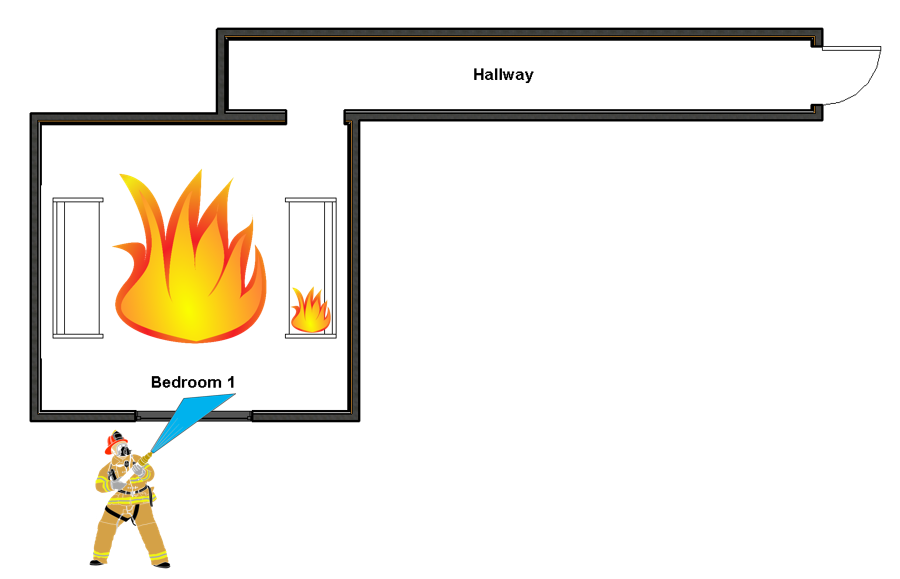
\includegraphics[width=5in]{Howard_Exp_1.png}
	\caption{Fire Experiment 1 Configuration}
	\label{fig:Exp1Config}
\end{figure}

\begin{table}[H]
	\centering
	\caption{Fire Experiment 1 Interventions}
	\begin{tabular}{|c|c|} 
		\hline
		Time & Intervention \\ \hline \hline
		00:00 & Ignition -- Bedroom \\ \hline
		04:30 & Exterior Suppression \\ \hline
		13:00 & End Experiment\\ \hline
	\end{tabular}
	\label{Table:Exp1Interventions}
\end{table}

\clearpage

\paragraph{Fire Experiment 2} \mbox{}

Fire Experiment 2 was a room and contents fire in the bedroom of the structure testing the ability for the fire to regrow after an exterior attack. This test was similar to Fire Experiment 1 with the exception of additional fuel loading in the fire room. The details of the differences in the fuel loading can be found in the Fuel Load section above. The door to the hallway and the bedroom window within the structure were open for the duration of the test. The fire was allowed to grow to steady state before suppression. Suppression was conducted from the exterior of the structure via a straight stream on a 150~gpm at 75~psi combination nozzle connected to a 1~3/4~in hoseline. The nozzle firefighter was positioned close to the window opening and the hose stream was directed at the ceiling via a max angle position. Water was applied for approximately 10 seconds. After 16 minutes, it was determined that the fire was not going to re-grow and thus was re-ignited manually in the bedroom and was allowed to grow uninhibited once again until a steady state condition was reached. Exterior suppression was completed as before with water flowing for approximately 8 seconds. After approximately 14 minutes, the fire re-grew to a new steady state and was suppressed one last time using the same method as above with water flowing for approximately 10 seconds. Figure~\ref{fig:Exp2Config} shows the configuration of the structure and Table~\ref{Table:Exp2Interventions} shows at what times interventions were performed.  

% The results of Fire Experiment 1 can be found in Appendix~\ref{App:Exp1Results}. To view the full experiment video \href{https://youtu.be/gl8rc1Nsl1k}{Click Here}.

\begin{figure}[H]
	\centering
	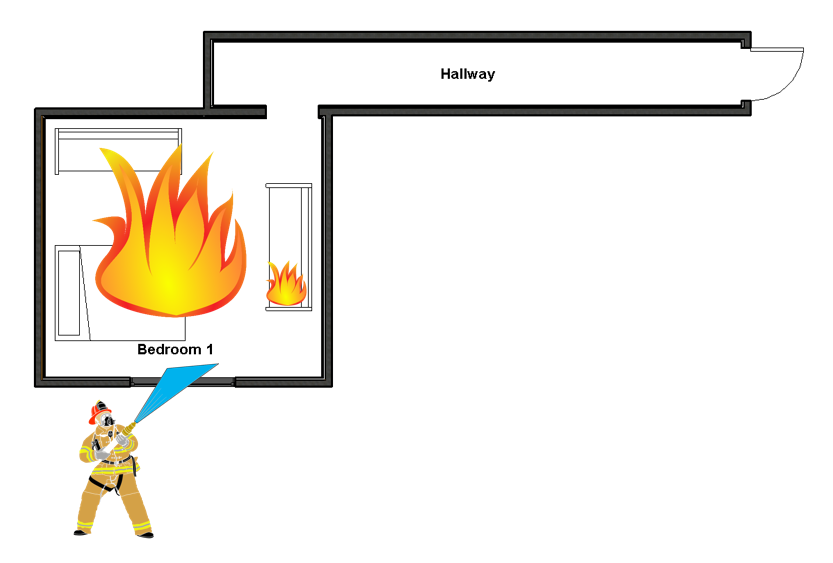
\includegraphics[width=5in]{Howard_Exp_2.png}
	\caption{Fire Experiment 2 Configuration}
	\label{fig:Exp2Config}
\end{figure}

\begin{table}[H]
	\centering
	\caption{Fire Experiment 2 Interventions}
	\begin{tabular}{|c|c|} 
		\hline
		Time & Intervention \\ \hline \hline
		00:00 & Ignition -- Bedroom \\ \hline
		05:00 & Exterior Suppression \\ \hline
		21:00 & Second Ignition -- Bedroom \\ \hline
		27:00 & Exterior Suppression \\ \hline
		40:20 & Exterior Suppression \\ \hline
		44:00 & End Experiment\\ \hline
	\end{tabular}
	\label{Table:Exp2Interventions}
\end{table}

\clearpage

\paragraph{Fire Experiment 3} \mbox{}

Fire Experiment 3 was a room and contents fire in the bedroom of the structure testing the impact of hose stream air entrainment on fire behavior and suppression capability. The door to the hallway and the bedroom window within the structure were open for the duration of the test. The fire was allowed to grow to steady state before suppression. Suppression was conducted from the interior of the structure via a straight stream on a 150~gpm at 75~psi combination nozzle connected to a 1~3/4~in hoseline. The nozzle firefighter advanced down the hallway and the hose stream was directed ahead in a wall-ceiling-wall pattern before entering the fire room for final extinguishment. Figure~\ref{fig:Exp3Config} shows the configuration of the structure and Table~\ref{Table:Exp3Interventions} shows at what times interventions were performed.  

% The results of Fire Experiment 1 can be found in Appendix~\ref{App:Exp1Results}. To view the full experiment video \href{https://youtu.be/gl8rc1Nsl1k}{Click Here}.

\begin{figure}[H]
	\centering
	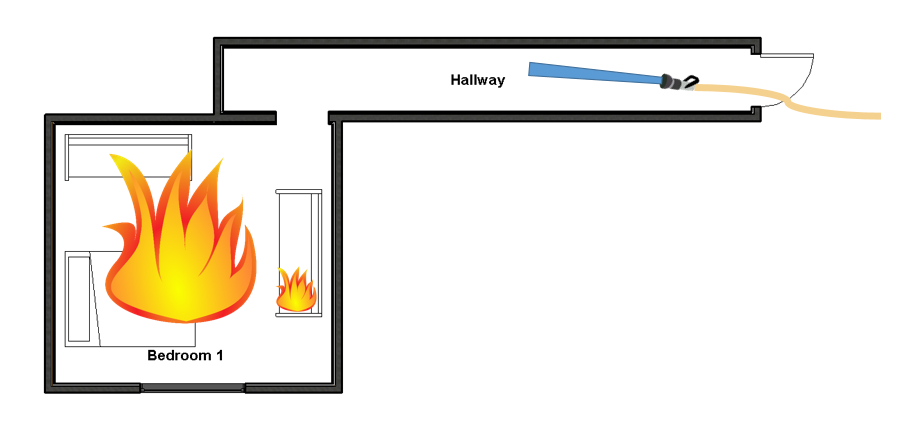
\includegraphics[width=5in]{Howard_Exp_3.png}
	\caption{Fire Experiment 3 Configuration}
	\label{fig:Exp3Config}
\end{figure}

\begin{table}[H]
	\centering
	\caption{Fire Experiment 3 Interventions}
	\begin{tabular}{|c|c|} 
		\hline
		Time & Intervention \\ \hline \hline
		00:00 & Ignition -- Bedroom \\ \hline
		05:00 & Interior Suppression \\ \hline
		15:00 & End Experiment\\ \hline
	\end{tabular}
	\label{Table:Exp3Interventions}
\end{table}

\clearpage

\paragraph{Fire Experiment 4} \mbox{}

Fire Experiment 4 was a room and contents fire in the bedroom of the structure testing the impact of hose stream air entrainment on fire behavior and suppression capability. The door to the hallway and the bedroom window within the structure were open for the duration of the test. The fire was allowed to grow to steady state before suppression. Suppression was conducted from the interior of the structure via a narrow fog stream on a 150~gpm at 75~psi combination nozzle connected to a 1~3/4~in hoseline. The nozzle firefighter advanced down the hallway and the hose stream was directed ahead in an `O' pattern before entering the fire room for final extinguishment. Figure~\ref{fig:Exp4Config} shows the configuration of the structure and Table~\ref{Table:Exp4Interventions} shows at what times interventions were performed. 

% The results of Fire Experiment 1 can be found in Appendix~\ref{App:Exp1Results}. To view the full experiment video \href{https://youtu.be/gl8rc1Nsl1k}{Click Here}.

\begin{figure}[H]
	\centering
	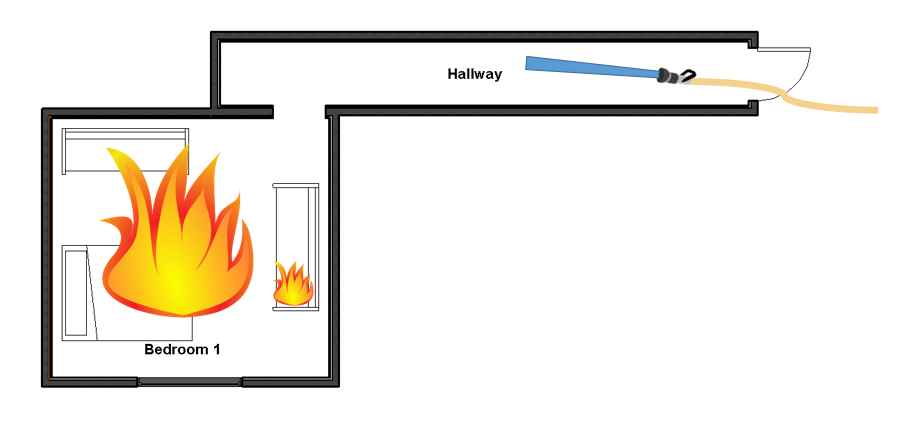
\includegraphics[width=5in]{Howard_Exp_4.png}
	\caption{Fire Experiment 4 Configuration}
	\label{fig:Exp4Config}
\end{figure}

\begin{table}[H]
	\centering
	\caption{Fire Experiment 4 Interventions}
	\begin{tabular}{|c|c|} 
		\hline
		Time & Intervention \\ \hline \hline
		00:00 & Ignition -- Bedroom \\ \hline
		07:30 & Interior Suppression \\ \hline
		14:00 & End Experiment\\ \hline
	\end{tabular}
	\label{Table:Exp4Interventions}
\end{table}

\clearpage

\paragraph{Fire Experiment 5} \mbox{}

Fire Experiment 5 was a room and contents fire in the bedroom of the structure testing the impact of door control. The bedroom window within the structure was open for the duration of the test. The fire was allowed to grow to steady state before the hall door was manipulated from the exterior of the structure. Several iterations of door open and door closed were performed before suppression. Suppression was conducted from the exterior of the structure via a straight stream on a 150~gpm at 75~psi combination nozzle connected to a 1~3/4~in hoseline. The nozzle firefighter was positioned close to the window opening and the hose stream was directed at the ceiling via a max angle position. Water was applied for approximately 10 seconds. Figure~\ref{fig:Exp5Config} shows the configuration of the structure and Table~\ref{Table:Exp5Interventions} shows at what times interventions were performed.

% The results of Fire Experiment 1 can be found in Appendix~\ref{App:Exp1Results}. To view the full experiment video \href{https://youtu.be/gl8rc1Nsl1k}{Click Here}.

\begin{figure}[H]
	\centering
	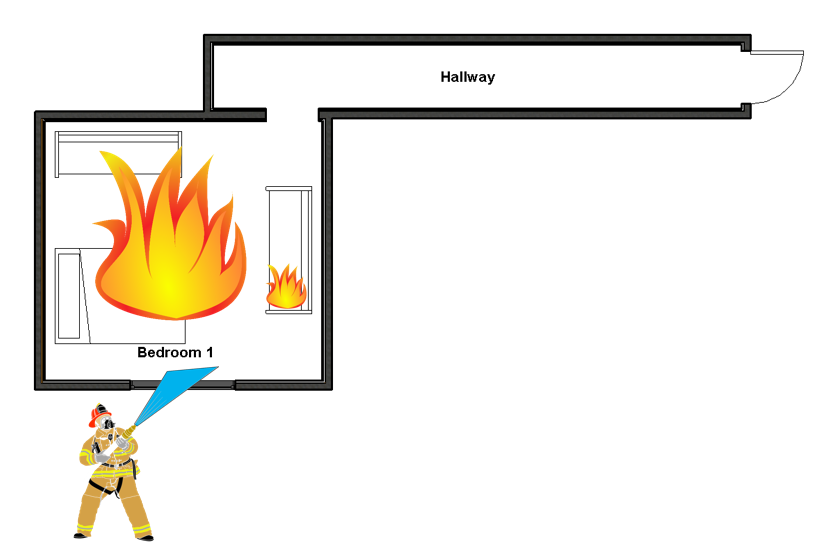
\includegraphics[width=5in]{Howard_Exp_5.png}
	\caption{Fire Experiment 5 Configuration}
	\label{fig:Exp5Config}
\end{figure}

\begin{table}[H]
	\centering
	\caption{Fire Experiment 5 Interventions}
	\begin{tabular}{|c|c|} 
		\hline
		Time & Intervention \\ \hline \hline
		00:00 & Ignition -- Bedroom \\ \hline
		04:30 & Hall Door Closed \\ \hline
		05:00 & Hall Door Open \\ \hline
		06:00 & Hall Door Closed \\ \hline
		07:00 & Hall Door Open \\ \hline
		08:00 & Hall Door Closed \\ \hline
		09:00 & Hall Door Open \\ \hline
		11:00 & Exterior Suppression \\ \hline
		20:00 & End Experiment\\ \hline
	\end{tabular}
	\label{Table:Exp5Interventions}
\end{table}

\clearpage

\paragraph{Fire Experiment 6} \mbox{}

Fire Experiment 6 was a room and contents fire in the bedroom of the structure testing the impact of door control. The bedroom window within the structure was closed for the duration of the test. The fire was allowed to grow to steady state before the hall door was manipulated from the exterior of the structure. Several iterations of door open and door closed were performed before the bedroom window was ventilated from the exterior. Additional manipulations of the hall door followed ventilation and before interior suppression was conducted. Suppression was conducted from the interior of the structure via a straight stream on a 150~gpm at 75~psi combination nozzle connected to a 1~3/4~in hoseline. The nozzle firefighter advanced down the hallway and the hose stream was directed ahead in a wall-ceiling-wall pattern before entering the fire room for final extinguishment. Figure~\ref{fig:Exp6Config} shows the configuration of the structure and Table~\ref{Table:Exp6Interventions} shows at what times interventions were performed.

% The results of Fire Experiment 1 can be found in Appendix~\ref{App:Exp1Results}. To view the full experiment video \href{https://youtu.be/gl8rc1Nsl1k}{Click Here}.

\begin{figure}[H]
	\centering
	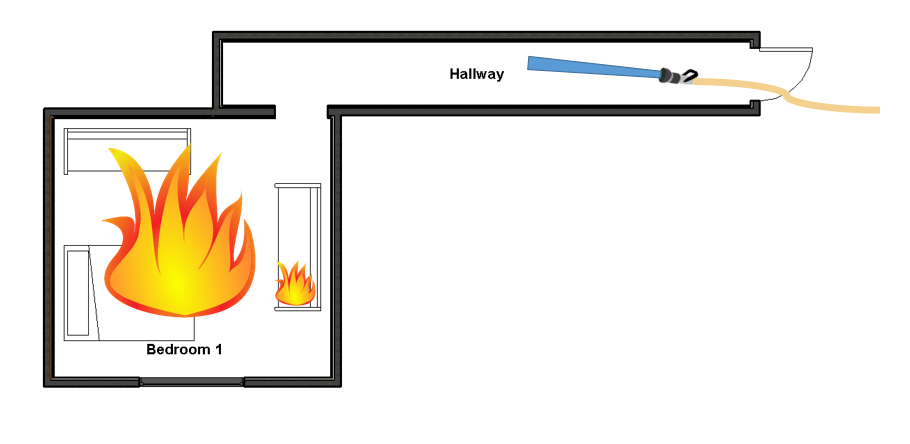
\includegraphics[width=5in]{Howard_Exp_6.png}
	\caption{Fire Experiment 6 Configuration}
	\label{fig:Exp6Config}
\end{figure}

\begin{table}[H]
	\centering
	\caption{Fire Experiment 6 Interventions}
	\begin{tabular}{|c|c|} 
		\hline
		Time & Intervention \\ \hline \hline
		00:00 & Ignition -- Bedroom \\ \hline
		04:00 & Hall Door Closed \\ \hline
		04:30 & Hall Door Open \\ \hline
		05:30 & Hall Door Closed \\ \hline
		06:30 & Hall Door Open \\ \hline
		11:30 & Second Ignition -- Bedroom \\ \hline
		16:45 & Hall Door Closed \\ \hline
		17:15 & Hall Door Open \\ \hline
		19:45 & Hall Door Closed \\ \hline
		20:15 & Hall Door Open \\ \hline
		21:00 & Bedroom Window Vent \\ \hline
		23:30 & Interior Suppression \\ \hline
		35:00 & End Experiment\\ \hline
	\end{tabular}
	\label{Table:Exp6Interventions}
\end{table}

\clearpage

\chapter{Results and Discussion}

\section*{Air Entrainment from Hose Streams}

\paragraph{Effect of Vent Ahead of Hose Stream} \mbox{}

Experiments~1--3 followed an identical sequence of events. During Experiments~1 and 2, the window in Bedroom~1 was opened. During Experiment~3, however, the Bedroom~1 window was closed, removing the vent opening ahead of the hose stream. Figs.~\ref{fig:Exps1_and_2_bar_graph} and \ref{fig:Exp3_bar_graph} contain bar graphs of the average flow in CFM through the hallway door during the different configurations tested for Experiments~1 and~2 and Experiment~3, respectively. Note, negative CFM is indicative of flow down the hall and out the structure through the hall doorway, and positive CFM is indicative of flow in the opposite direction: into the structure through the hall doorway.

\begin{figure}[!ht]
	\centering
	\includegraphics[width=\columnwidth]{../2_Plots/Ent_Experiment_Plots/Bar_Graphs/Experiments_1+2_hall_locations}
	\caption{Average air flow in CFM through hall entrance doorway (positive values indicate flow through doorway and into the structure towards the bedroom) for the different configurations tested during Experiments~1 and~2.}
	\label{fig:Exps1_and_2_bar_graph}
\end{figure}

\begin{figure}[!ht]
	\centering
	\includegraphics[width=\columnwidth]{../2_Plots/Ent_Experiment_Plots/Bar_Graphs/Experiment_3_hall_locations}
	\caption{Average air flow in CFM through hall entrance doorway (positive values indicate flow through doorway and into the structure towards the bedroom) for the different configurations tested during Experiment~3.}
	\label{fig:Exp3_bar_graph}
\end{figure}

Looking at the two figures, it can be seen that a vent ahead of the hose stream can have a drastic effect on air movement in the structure. With no vent present, the amount of air flow out of the structure through the hall doorway increased significantly. This can be attributed to the fact that the hall doorway was the only vent opening present. When the bedroom window was opened, providing an additional vent, air flow through the hall doorway decreased because the second opening helped relieve pressure. Furthermore, while applying a narrow fog in an `O' pattern at the start of the hallway and middle of the hallway and a vent opened ahead (Fig.~\ref{fig:Exps1_and_2_bar_graph}), the average flow through the hall doorway is positive, meaning that the hose stream is causing air to be entrained through the doorway in the direction of towards the bedroom. [SENTENCE ABOUT POSITION IN HALL?]

\FloatBarrier

\paragraph{Effect of Increasing Stream Length Flowing into Window} \mbox{}

Between Experiments~5, 6, 12, and 13, a fixed straight stream was applied into the bedroom through the window from the following locations: at the edge of the window, 6~ft from the window, 12~ft from the window, 24~ft from the window, and 48~ft from the window. Fig.~\ref{fig:Exps5_6_12_and_13_bar_graph} contains a bar graph of the average flow of air through the hall door in CFM during the straight stream application at these distances. In the provided figure, a positive CFM value is indicative of flow through the hall doorway and out the structure.

\begin{figure}[!ht]
	\centering
	\includegraphics[width=\columnwidth]{../2_Plots/Ent_Experiment_Plots/Bar_Graphs/Experiments_5+6_12+13_five_distances_from_window}
	\caption{Average CFM through hall door while applying straight stream into the bedroom through the window from locations of at the Window, 6~ft from the window, 12~ft from the window, 24~ft from the window, and 48~ft from the window.}
	\label{fig:Exps5_6_12_and_13_bar_graph}
\end{figure}

Overall, from Fig.~\ref{fig:Exps5_6_12_and_13_bar_graph}, it was observed that more distance between the nozzle and the window, the more air flow through the hall doorway. This occurs because as the length of the hose stream increases, the spread of water droplets at the end of the stream increases. 

\FloatBarrier

\paragraph{Flow from Hallway into Bedroom} \mbox{}

Experiment~4 involved flowing water in a straight stream and narrow fog stream from the end of the hallway into the bedroom. Fig.~\ref{fig:Exp4_three targets_bar_graph} compares the average CFM through entrance doorway to the hall for the two streams applied in a fixed manner and in an `O' pattern aimed at max angle, mid ceiling, and out the window. Fig.~\ref{fig:Exp4_sweeping_bar_graph} contains a similar bar graph comparing the average flow in CFM through the same doorway for a straight stream and narrow fog applied from the hallway into the bedroom in a sweeping pattern. For both figures, positive CFM values indicate flow from the exterior through the entrance doorway of the hall and towards the bedroom [REFERENCE TO EXP DESCRIPTION]. 

\begin{figure}[!ht]
	\centering
	\includegraphics[width=\columnwidth]{../2_Plots/Ent_Experiment_Plots/Bar_Graphs/Experiment_4_three_targets_BR1_door}
	\caption{Average air flow in CFM through hallway door (positive flow is into the structure through the doorway and down the hallway towards the bedroom) while applying a straight stream and narrow fog in a fixed position and an `O' pattern from the end of the hallway into the bedroom aimed at max angle, mid ceiling, and out the window.}
	\label{fig:Exp4_three targets_bar_graph}
\end{figure}

\begin{figure}[!ht]
	\centering
	\includegraphics[width=\columnwidth]{../2_Plots/Ent_Experiment_Plots/Bar_Graphs/Experiment_4_sweeping_BR1_door}
	\caption{Average air flow in CFM through hallway door (positive flow is into the structure through the doorway and down the hallway towards the bedroom) while applying a straight stream and narrow fog in a sweeping pattern from the end of the hallway into the bedroom.}
	\label{fig:Exp4_sweeping_bar_graph}
\end{figure}

Figs.~\ref{fig:Exp4_three targets_bar_graph} and~\ref{fig:Exp4_sweeping_bar_graph} show that entrainment occurred through the hall doorway during the application of the straight stream in an `O' pattern and both applications of the narrow fog aimed out the window. Additionally, the narrow fog entrained significantly more air compared to the straight stream in an `O' pattern. This result is reasonable as the configuration simulates hydraulic ventilation described in [REFER TO EARLIER EXPLANATION]. Flowing water with the stream aimed at max angle and mid ceiling did not cause entrainment through the hallway entrance door for any of the hose stream and application pattern combinations. The only other hose stream and application pattern combination that caused air to flow from the exterior through the hall doorway towards the bedroom was the narrow fog in a sweeping pattern.

\FloatBarrier

\paragraph{Straight Stream and Smooth Bore Comparison} \mbox{}

During Experiments~8 and~9, a combination nozzle set to straight stream was used to apply water through the bedroom window from the exterior of the structure at the `max angle' position with the hose stream fixed and with the sweeping pattern. During Experiments~10 and~11, a smooth bore nozzle with a 7/8~in tip was used to apply water in an identical manner. Fig.~\ref{fig:Exps8_9_10_and_11_bar_graph} contains a bar graph of the average air flow in CFM through the hallway door for each of the configurations. Note, positive flow is in the direction of through the doorway to the exterior of the structure. 

\begin{figure}[!ht]
	\centering
	\includegraphics[width=\columnwidth]{../2_Plots/Ent_Experiment_Plots/Bar_Graphs/Experiments_8+9_10+11_max_angle}
	\caption{Average air flow in CFM through hall door (positive flow is through the doorway to the exterior of the structure) while applying a straight stream and stream from a smooth bore nozzle into the bedroom through the window at the max angle position in a fixed position and sweeping pattern.}
	\label{fig:Exps8_9_10_and_11_bar_graph}
\end{figure}

From Fig.~\ref{fig:Exps8_9_10_and_11_bar_graph}, the amount of air flow caused by the straight stream is indistinguishable (i.e., within the uncertainty bounds of) from the amount of air flow caused by the stream from the smooth bore nozzle.

Additionally, during Experiments~8 and~9, a narrow fog was applied into the bedroom from the same position using the ``whip'' pattern. A stream from the smooth bore nozzle with the bale half opened was applied in an identical manner during Experiments~10 and~11. Looking at Fig.~\ref{fig:Exps8_9_10_and_11_whip_bar_graph}, which contains a bar graph of the average flow through the hall doorway in CFM for the two streams applied in the ``whip'' pattern, no noticeable differences between the amount of flow through the hallway door caused by the two configurations were observed.

\begin{figure}[!ht]
	\centering
	\includegraphics[width=\columnwidth]{../2_Plots/Ent_Experiment_Plots/Bar_Graphs/Experiments_8+9_10+11_whip}
	\caption{Average air flow in CFM through hall door (positive flow is through the doorway to the exterior of the structure) while applying a narrow fog and stream from a smooth bore nozzle with the bale opened half way into the bedroom through the window in the ``whip'' pattern.}
	\label{fig:Exps8_9_10_and_11_whip_bar_graph}
\end{figure}

\FloatBarrier

\paragraph{Straight Stream and Narrow Fog Comparison} \mbox{}

In general, the narrow fog stream produced greater air flow through the hall entrance doorway than the straight stream for the different configurations. Referring back to Fig.~\ref{fig:Exps1_and_2_bar_graph}, air entrainment, or flow into the structure, occurred during Experiments~1 and~2 for only two configurations: the narrow fog applied in the `O' pattern at the start of the hallway and at the middle of the hallway. Comparing the average CFM value of the straight stream in the fixed position to the average CFM value of the narrow fog in the fixed position and the average CFM value of the straight stream being applied in a moving pattern (WCW) [INCLUDE APPLICATION PATTERN EXPLANATIONS IN EARLIER SECTION] to the average value of the narrow fog being applied in a moving pattern (`O'), the magnitude of the average CFM was always larger for the narrow fog stream, indicating that the narrow fog caused more air movement than the straight stream. [ANYTHING ABOUT EXPERIMENT 3 HERE?] 

In addition to flowing a fixed straight stream through the bedroom window from the exterior of the structure at locations of at the window, 6~ft from the window, and 12~ft from the window, a straight stream in the `O' pattern, a narrow fog in the fixed pattern, and a narrow fog in the `O' pattern were also applied in a similar manner. Fig.~\ref{fig:Exps5_and_6_three_distances} contains a bar graph of the average air flow in CFM for each configuration tested during Experiments~5 and~6. In the provided figure, positive CFM values indicate air flow in the direction of down the hall through the hall entrance doorway and out to the exterior.

\begin{figure}[!ht]
	\centering
	\includegraphics[width=\columnwidth]{../2_Plots/Ent_Experiment_Plots/Bar_Graphs/Experiments_5+6_three_distances_from_window}
	\caption{Average air flow in CFM through hall door (positive flow is through the doorway to the exterior of the structure) while applying a narrow fog and stream from a smooth bore nozzle with the bale opened half way into the bedroom through the window in the ``whip'' pattern.}
	\label{fig:Exps5_and_6_three_distances}
\end{figure}

Comparing the average CFM values produced by the straight stream and narrow fog stream applied in the fixed position and in the `O' pattern, the average CFM of air flow produced by the narrow fog was always greater in magnitude compared to the corresponding CFM generated by the straight stream.

\FloatBarrier

% \begin{appendices}
% \section*{Experimental Results} \label{App:Results}

% \subsection*{Experiment 1}
% \label{app:Experiment_1}

% \begin{figure}[!ht]
% \begin{tabular*}{\textwidth}{lr}
% \includegraphics[width=0.45\columnwidth]{../2_Plots/Fire_Experiment_Plots/Experiment_1_Data/Bedroom_1_Temps.png} &
% \includegraphics[width=0.45\columnwidth]{../2_Plots/Fire_Experiment_Plots/Experiment_1_Data/End_Hall_Temps.png} \\
% \includegraphics[width=0.45\columnwidth]{../2_Plots/Fire_Experiment_Plots/Experiment_1_Data/Mid_Hall_Temps.png} &
% \includegraphics[width=0.45\columnwidth]{../2_Plots/Fire_Experiment_Plots/Experiment_1_Data/Start_Hall_Temps.png} \\
% \end{tabular*}
% \caption[Experiment 1 Temperatures]{Temperature data for Experiment 1 in the bedroom, end hall, mid hall, and start hall positions.}
% \end{figure}

% \clearpage

% \begin{figure}[!ht]
% \begin{tabular*}{\textwidth}{lr}
% \includegraphics[width=0.45\columnwidth]{../2_Plots/Fire_Experiment_Plots/Experiment_1_Data/Bedroom_1_Window.png} &
% \includegraphics[width=0.45\columnwidth]{../2_Plots/Fire_Experiment_Plots/Experiment_1_Data/Bedroom_1_Inside_Door.png} \\
% \includegraphics[width=0.45\columnwidth]{../2_Plots/Fire_Experiment_Plots/Experiment_1_Data/Bedroom_1_Outside_Door.png} &
% \includegraphics[width=0.45\columnwidth]{../2_Plots/Fire_Experiment_Plots/Experiment_1_Data/Start_Hall_Door.png} \\
% \end{tabular*}
% \caption[Experiment 1 Gas Flows]{Gas flow data for Experiment 1 in the bedroom, inside door, outside door, and start hall positions.}
% \end{figure}

% \clearpage

% \begin{figure}[!ht]
% \begin{tabular*}{\textwidth}{lr}
% \includegraphics[width=0.45\columnwidth]{../2_Plots/Fire_Experiment_Plots/Experiment_1_Data/Bedroom_1_Pressure.png} &
% \includegraphics[width=0.45\columnwidth]{../2_Plots/Fire_Experiment_Plots/Experiment_1_Data/Hallway_Pressure.png} \\
% \end{tabular*}
% \caption[Experiment 1 Pressures]{Pressure data for Experiment 1 in the bedroom and hallway positions.}
% \end{figure}

% \clearpage

% \subsection*{Experiment 2}
% \label{app:Experiment_2}

% \begin{figure}[!ht]
% \begin{tabular*}{\textwidth}{lr}
% \includegraphics[width=0.45\columnwidth]{../2_Plots/Fire_Experiment_Plots/Experiment_2_Data/Bedroom_1_Temps.png} &
% \includegraphics[width=0.45\columnwidth]{../2_Plots/Fire_Experiment_Plots/Experiment_2_Data/End_Hall_Temps.png} \\
% \includegraphics[width=0.45\columnwidth]{../2_Plots/Fire_Experiment_Plots/Experiment_2_Data/Mid_Hall_Temps.png} &
% \includegraphics[width=0.45\columnwidth]{../2_Plots/Fire_Experiment_Plots/Experiment_2_Data/Start_Hall_Temps.png} \\
% \end{tabular*}
% \caption[Experiment 2 Temperatures]{Temperature data for Experiment 2 in the bedroom, end hall, mid hall, and start hall positions.}
% \end{figure}

% \clearpage

% \begin{figure}[!ht]
% \begin{tabular*}{\textwidth}{lr}
% \includegraphics[width=0.45\columnwidth]{../2_Plots/Fire_Experiment_Plots/Experiment_2_Data/Bedroom_1_Window.png} &
% \includegraphics[width=0.45\columnwidth]{../2_Plots/Fire_Experiment_Plots/Experiment_2_Data/Bedroom_1_Inside_Door.png} \\
% \includegraphics[width=0.45\columnwidth]{../2_Plots/Fire_Experiment_Plots/Experiment_2_Data/Bedroom_1_Outside_Door.png} &
% \includegraphics[width=0.45\columnwidth]{../2_Plots/Fire_Experiment_Plots/Experiment_2_Data/Start_Hall_Door.png} \\
% \end{tabular*}
% \caption[Experiment 2 Gas Flows]{Gas flow data for Experiment 2 in the bedroom, inside door, outside door, and start hall positions.}
% \end{figure}

% \clearpage

% \begin{figure}[!ht]
% \begin{tabular*}{\textwidth}{lr}
% \includegraphics[width=0.45\columnwidth]{../2_Plots/Fire_Experiment_Plots/Experiment_2_Data/Bedroom_1_Pressure.png} &
% \includegraphics[width=0.45\columnwidth]{../2_Plots/Fire_Experiment_Plots/Experiment_2_Data/Hallway_Pressure.png} \\
% \end{tabular*}
% \caption[Experiment 2 Pressures]{Pressure data for Experiment 2 in the bedroom and hallway positions.}
% \end{figure}

% \clearpage

% \subsection*8{Experiment 3}
% \label{app:Experiment_3}

% \begin{figure}[!ht]
% \begin{tabular*}{\textwidth}{lr}
% \includegraphics[width=0.45\columnwidth]{../2_Plots/Fire_Experiment_Plots/Experiment_3_Data/Bedroom_1_Temps.png} &
% \includegraphics[width=0.45\columnwidth]{../2_Plots/Fire_Experiment_Plots/Experiment_3_Data/End_Hall_Temps.png} \\
% \includegraphics[width=0.45\columnwidth]{../2_Plots/Fire_Experiment_Plots/Experiment_3_Data/Mid_Hall_Temps.png} &
% \includegraphics[width=0.45\columnwidth]{../2_Plots/Fire_Experiment_Plots/Experiment_3_Data/Start_Hall_Temps.png} \\
% \end{tabular*}
% \caption[Experiment 3 Temperatures]{Temperature data for Experiment 3 in the bedroom, end hall, mid hall, and start hall positions.}
% \end{figure}

% \clearpage

% \begin{figure}[!ht]
% \begin{tabular*}{\textwidth}{lr}
% \includegraphics[width=0.45\columnwidth]{../2_Plots/Fire_Experiment_Plots/Experiment_3_Data/Bedroom_1_Window.png} &
% \includegraphics[width=0.45\columnwidth]{../2_Plots/Fire_Experiment_Plots/Experiment_3_Data/Bedroom_1_Inside_Door.png} \\
% \includegraphics[width=0.45\columnwidth]{../2_Plots/Fire_Experiment_Plots/Experiment_3_Data/Bedroom_1_Outside_Door.png} &
% \includegraphics[width=0.45\columnwidth]{../2_Plots/Fire_Experiment_Plots/Experiment_3_Data/Start_Hall_Door.png} \\
% \end{tabular*}
% \caption[Experiment 3 Gas Flows]{Gas flow data for Experiment 3 in the bedroom, inside door, outside door, and start hall positions.}
% \end{figure}

% \clearpage

% \begin{figure}[!ht]
% \begin{tabular*}{\textwidth}{lr}
% \includegraphics[width=0.45\columnwidth]{../2_Plots/Fire_Experiment_Plots/Experiment_3_Data/Bedroom_1_Pressure.png} &
% \includegraphics[width=0.45\columnwidth]{../2_Plots/Fire_Experiment_Plots/Experiment_3_Data/Hallway_Pressure.png} \\
% \end{tabular*}
% \caption[Experiment 3 Pressures]{Pressure data for Experiment 3 in the bedroom and hallway positions.}
% \end{figure}

% \clearpage

% \subsection*8{Experiment 4}
% \label{app:Experiment_4}

% \begin{figure}[!ht]
% \begin{tabular*}{\textwidth}{lr}
% \includegraphics[width=0.45\columnwidth]{../2_Plots/Fire_Experiment_Plots/Experiment_4_Data/Bedroom_1_Temps.png} &
% \includegraphics[width=0.45\columnwidth]{../2_Plots/Fire_Experiment_Plots/Experiment_4_Data/End_Hall_Temps.png} \\
% \includegraphics[width=0.45\columnwidth]{../2_Plots/Fire_Experiment_Plots/Experiment_4_Data/Mid_Hall_Temps.png} &
% \includegraphics[width=0.45\columnwidth]{../2_Plots/Fire_Experiment_Plots/Experiment_4_Data/Start_Hall_Temps.png} \\
% \end{tabular*}
% \caption[Experiment 4 Temperatures]{Temperature data for Experiment 4 in the bedroom, end hall, mid hall, and start hall positions.}
% \end{figure}

% \clearpage

% \begin{figure}[!ht]
% \begin{tabular*}{\textwidth}{lr}
% \includegraphics[width=0.45\columnwidth]{../2_Plots/Fire_Experiment_Plots/Experiment_4_Data/Bedroom_1_Window.png} &
% \includegraphics[width=0.45\columnwidth]{../2_Plots/Fire_Experiment_Plots/Experiment_4_Data/Bedroom_1_Inside_Door.png} \\
% \includegraphics[width=0.45\columnwidth]{../2_Plots/Fire_Experiment_Plots/Experiment_4_Data/Bedroom_1_Outside_Door.png} &
% \includegraphics[width=0.45\columnwidth]{../2_Plots/Fire_Experiment_Plots/Experiment_4_Data/Start_Hall_Door.png} \\
% \end{tabular*}
% \caption[Experiment 4 Gas Flows]{Gas flow data for Experiment 4 in the bedroom, inside door, outside door, and start hall positions.}
% \end{figure}

% \clearpage

% \begin{figure}[!ht]
% \begin{tabular*}{\textwidth}{lr}
% \includegraphics[width=0.45\columnwidth]{../2_Plots/Fire_Experiment_Plots/Experiment_4_Data/Bedroom_1_Pressure.png} &
% \includegraphics[width=0.45\columnwidth]{../2_Plots/Fire_Experiment_Plots/Experiment_4_Data/Hallway_Pressure.png} \\
% \end{tabular*}
% \caption[Experiment 4 Pressures]{Pressure data for Experiment 4 in the bedroom and hallway positions.}
% \end{figure}

% \clearpage

% \subsection*8{Experiment 5}
% \label{app:Experiment_5}

% \begin{figure}[!ht]
% \begin{tabular*}{\textwidth}{lr}
% \includegraphics[width=0.45\columnwidth]{../2_Plots/Fire_Experiment_Plots/Experiment_5_Data/Bedroom_1_Temps.png} &
% \includegraphics[width=0.45\columnwidth]{../2_Plots/Fire_Experiment_Plots/Experiment_5_Data/End_Hall_Temps.png} \\
% \includegraphics[width=0.45\columnwidth]{../2_Plots/Fire_Experiment_Plots/Experiment_5_Data/Mid_Hall_Temps.png} &
% \includegraphics[width=0.45\columnwidth]{../2_Plots/Fire_Experiment_Plots/Experiment_5_Data/Start_Hall_Temps.png} \\
% \end{tabular*}
% \caption[Experiment 5 Temperatures]{Temperature data for Experiment 5 in the bedroom, end hall, mid hall, and start hall positions.}
% \end{figure}

% \clearpage

% \begin{figure}[!ht]
% \begin{tabular*}{\textwidth}{lr}
% \includegraphics[width=0.45\columnwidth]{../2_Plots/Fire_Experiment_Plots/Experiment_5_Data/Bedroom_1_Window.png} &
% \includegraphics[width=0.45\columnwidth]{../2_Plots/Fire_Experiment_Plots/Experiment_5_Data/Bedroom_1_Inside_Door.png} \\
% \includegraphics[width=0.45\columnwidth]{../2_Plots/Fire_Experiment_Plots/Experiment_5_Data/Bedroom_1_Outside_Door.png} &
% \includegraphics[width=0.45\columnwidth]{../2_Plots/Fire_Experiment_Plots/Experiment_5_Data/Start_Hall_Door.png} \\
% \end{tabular*}
% \caption[Experiment 5 Gas Flows]{Gas flow data for Experiment 5 in the bedroom, inside door, outside door, and start hall positions.}
% \end{figure}

% \clearpage

% \begin{figure}[!ht]
% \begin{tabular*}{\textwidth}{lr}
% \includegraphics[width=0.45\columnwidth]{../2_Plots/Fire_Experiment_Plots/Experiment_5_Data/Bedroom_1_Pressure.png} &
% \includegraphics[width=0.45\columnwidth]{../2_Plots/Fire_Experiment_Plots/Experiment_5_Data/Hallway_Pressure.png} \\
% \end{tabular*}
% \caption[Experiment 5 Pressures]{Pressure data for Experiment 5 in the bedroom and hallway positions.}
% \end{figure}

% \clearpage

% \subsection*{Experiment 6}
% \label{app:Experiment_6}

% \begin{figure}[!ht]
% \begin{tabular*}{\textwidth}{lr}
% \includegraphics[width=0.45\columnwidth]{../2_Plots/Fire_Experiment_Plots/Experiment_6_Data/Bedroom_1_Temps.png} &
% \includegraphics[width=0.45\columnwidth]{../2_Plots/Fire_Experiment_Plots/Experiment_6_Data/End_Hall_Temps.png} \\
% \includegraphics[width=0.45\columnwidth]{../2_Plots/Fire_Experiment_Plots/Experiment_6_Data/Mid_Hall_Temps.png} &
% \includegraphics[width=0.45\columnwidth]{../2_Plots/Fire_Experiment_Plots/Experiment_6_Data/Start_Hall_Temps.png} \\
% \end{tabular*}
% \caption[Experiment 6 Temperatures]{Temperature data for Experiment 6 in the bedroom, end hall, mid hall, and start hall positions.}
% \end{figure}

% \clearpage

% \begin{figure}[!ht]
% \begin{tabular*}{\textwidth}{lr}
% \includegraphics[width=0.45\columnwidth]{../2_Plots/Fire_Experiment_Plots/Experiment_6_Data/Bedroom_1_Window.png} &
% \includegraphics[width=0.45\columnwidth]{../2_Plots/Fire_Experiment_Plots/Experiment_6_Data/Bedroom_1_Inside_Door.png} \\
% \includegraphics[width=0.45\columnwidth]{../2_Plots/Fire_Experiment_Plots/Experiment_6_Data/Bedroom_1_Outside_Door.png} &
% \includegraphics[width=0.45\columnwidth]{../2_Plots/Fire_Experiment_Plots/Experiment_6_Data/Start_Hall_Door.png} \\
% \end{tabular*}
% \caption[Experiment 6 Gas Flows]{Gas flow data for Experiment 6 in the bedroom, inside door, outside door, and start hall positions.}
% \end{figure}

% \clearpage

% \begin{figure}[!ht]
% \begin{tabular*}{\textwidth}{lr}
% \includegraphics[width=0.45\columnwidth]{../2_Plots/Fire_Experiment_Plots/Experiment_6_Data/Bedroom_1_Pressure.png} &
% \includegraphics[width=0.45\columnwidth]{../2_Plots/Fire_Experiment_Plots/Experiment_6_Data/Hallway_Pressure.png} \\
% \end{tabular*}
% \caption[Experiment 6 Pressures]{Pressure data for Experiment 6 in the bedroom and hallway positions.}
% \end{figure}

% \clearpage

% \end{appendices}

\end{document}